\documentclass[]{report}
\usepackage{amsmath,amsfonts}
\usepackage{graphicx}
\usepackage{float}
\usepackage{url}
\usepackage{tikz}
\usepackage{amsmath}
\usepackage{booktabs}
\setcounter{MaxMatrixCols}{13}
\usepackage[hidelinks,hypertexnames=false]{hyperref}
\usetikzlibrary{arrows.meta, decorations.pathreplacing, decorations.pathmorphing}

% Title Page
\title{{\huge  Longitudinal Active Suspension Control in a Half-Car Model with Unsprang Masses} \\
	{\small Automatic Control\\
		Electronic Engineering for Intelligent Vehicles\\
		University of Bologna\\
		A.A. 2025-2026}}
\author{Alessandro Briccoli, Cristian Cecchini, Mario Di Marino}


\begin{document}

	
	\maketitle
	
	\begin{abstract}
		This report presents the modeling, design, and simulation of an active suspension control system aimed at improving ride comfort and handling performance in passenger vehicles. The study focuses on a half-car model that includes both front and rear suspension dynamics, allowing the analysis of vertical and pitch motion of the vehicle body. Unlike passive suspension systems, which rely solely on spring-damper elements, the active suspension system introduced here incorporates actuators capable of generating controlled forces to counteract road disturbances in real time.
		
		To achieve the desired ride quality, a control strategy based on Proportional-Integral-Derivative (PID) controllers is developed.  Additionally, a state estimation technique using a Kalman observer is incorporated to provide real-time estimates of the states, helping to adapt to acceleration and road profile in a faster and more effective way.
		
		The performance of the control system is evaluated through simulations conducted in MATLAB/Simulink. Results show a significant reduction in body acceleration and pitch angle variation when compared to a passive suspension system, demonstrating the effectiveness of the proposed approach in enhancing ride comfort. This project perfectly demonstrates, once again, the massive importance of active control strategies in automotive suspension design.
	\end{abstract}
	
	\chapter{Introduction}
\section{Motivations}
Suspension systems play a crucial role in ensuring vehicle stability, comfort, and safety. Traditional passive suspensions cannot adapt to changing road conditions, leading to undesired oscillations and reduced performance. 

In this project, focus on active suspension control in the longitudinal direction (front and rear), which aims to reduce vertical oscillations and pitch movements when the vehicle passes over bumps or uneven surfaces. The goal is to design a control system that keeps the car body as steady as possible, improving both passenger comfort and vehicle handling.

The half-car model was chosen because it provides a good trade-off between model simplicity and dynamic realism and allows to study the impact of front and rear suspension forces on the vehicle behavior without dealing with the complexity of a full 3D model.

	
%	\section{Contributions}
%	Describe what this project deals with. What has been done to solve the problem presented in the motivations.
	
%	\section{State of art and literature comparison}
%	List the closest works that deal with the same problem and compare the achievement obtained and the strategies exploited in %   this paper. For the search of the literature use \url{https://ieeexplore.ieee.org/Xplore/home.jsp} and  %      %\url{https://www.sciencedirect.com/}.
	
%	\section{Organisation of the manuscript}
%	Describe what the reader finds in each of the Sections of this manuscript.
	



\section{List of the symbols}
\begin{table}[H]
	\centering
	\caption{Symbol Table}
	\begin{tabular}{lll}
		\toprule
		\textbf{Symbol} & \textbf{Description} & \textbf{Dimension} \\
		\midrule
		$x$ & State vector & $\mathbb{R}^{12}$ \\
		$u$ & Control input vector $[u_1\;u_2]^T$ & $\mathbb{R}^{2}$ \\
		$y$ & Measured output vector & $\mathbb{R}^{5}$ \\
		$e$ & Control error vector & $\mathbb{R}^{2}$ \\
		$d$ & Disturbance vector & $\mathbb{R}^{6}$ \\
		$r$ & Reference vector $[r_z\; r_\theta]^T$ & $\mathbb{R}^{2}$ \\
		$\nu$ & Sensor noise vector & $\mathbb{R}^{5}$ \\
		$w$ & Exogenous input $w=\mathrm{col}(d,\nu,r)$ & --- \\
		
		$p_z$ & Vertical displacement of vehicle CoM & m \\
		$v_z$ & Vertical velocity of vehicle CoM & m/s \\
		$\theta$ & Pitch angle of vehicle body & rad \\
		$\dot{\theta}$ & Pitch angular velocity & rad/s \\
		
		$h_{wf}, h_{wr}$ & Front and rear wheel vertical displacement & m \\
		$\dot{h}_{wf}, \dot{h}_{wr}$ & Front and rear wheel vertical velocity & m/s \\
		
		$\theta_{gf}, \theta_{gr}$ & Road pitch angle at front and rear axle & rad \\
		$z_{gf}, z_{gr}$ & Road vertical displacement at front and rear axle & m \\
		
		$u_1$ & Total vertical actuator force & N \\
		$u_2$ & Pitch moment component of actuator input & Nm \\
		$f_{af}, f_{ar}$ & Front and rear actuator forces & N \\
		
		$d_f, d_r$ & Distance from CoM to front and rear axle & m \\
		$h_{cg}$ & Height of vehicle center of mass & m \\
		
		$m$ & Sprung mass (vehicle body) & kg \\
		$m_{wf}, m_{wr}$ & Front and rear unsprung mass & kg \\
		$J$ & Pitch moment of inertia & kg\,m$^2$ \\
		
		$k_f, k_r$ & Front and rear suspension stiffness & N/m \\
		$\beta_f, \beta_r$ & Front and rear suspension damping & N\,s/m \\
		
		$k_{tf}, k_{tr}$ & Front and rear tire stiffness & N/m \\
		
		$s_1, s_3$ & Front and rear suspension deflection & m \\
		$s_2, s_4$ & Front and rear suspension velocity & m/s \\
		
		$f_{sf}, f_{sr}$ & Front and rear suspension forces & N \\
		$f_{wf}, f_{wr}$ & Front and rear wheel dynamics forces & N \\
		
		$f_{x f}, f_{x r}$ & Longitudinal forces at front and rear axle & N \\
		$F_x$ & Total longitudinal force $F_x=f_{xf}+f_{xr}$ & N \\
		
		$f_2$ & Vertical acceleration of vehicle body & m/s$^2$ \\
		$f_4$ & Pitch angular acceleration & rad/s$^2$ \\
		
		$\alpha_{gf}, \alpha_{gr}$ & Road pitch angular acceleration (front, rear) & rad/s$^2$ \\
		$\dot{z}_{gf}, \dot{z}_{gr}$ & Road vertical velocity (front, rear) & m/s \\
		
		$y_x$ & Longitudinal accelerometer output & m/s$^2$ \\
		$y_z$ & Vertical accelerometer output & m/s$^2$ \\
		$y_\theta$ & Gyroscope pitch-rate measurement & rad/s \\
		$y_f, y_r$ & Front and rear suspension sensors & m \\
		
		$\nu_y, \nu_z, \nu_g, \nu_f, \nu_r$ & Sensor noise components & --- \\
		
		$r_z$ & Reference vertical position & m \\
		$r_\theta$ & Reference pitch angle & rad \\
		
		$g$ & Gravitational acceleration & m/s$^2$ \\
		$\gamma_f$ & Anti-Dive suspension inclination & --- \\
		$\gamma_r$ & Anti-Squat suspension inclination & --- \\
		\bottomrule
	\end{tabular}
\end{table}



	
%	\chapter{Active Suspensions Control System}
%
%	
%	\section{Model and Problem Formulation}
%	In this section, the formulation of the control problem for the active suspension system of a half-car model. This system aims to regulate both the vertical position and the perceived pitch angle of the vehicle body, enhancing ride comfort and handling. The model is described by a nonlinear dynamic system influenced by road disturbances, actuator forces, and sensor measurements.
%	
%	The general form of the system is expressed as:
%	\begin{align}
%		\dot{x} &= f(x, u, w) \\
%		y &= h(x, u, w) \\
%		e &= h_e(x, u, w)
%	\end{align}
%	
%	Where:
%	\begin{itemize}
%		\item $x \in \mathbb{R}^n$ is the \textbf{state vector},
%		\item $u \in \mathbb{R}^p$ is the \textbf{control input vector},
%		\item $y \in \mathbb{R}^q$ is the \textbf{measured output vector},
%		\item $e \in \mathbb{R}^{l_m}$ is the \textbf{control error (goal)},
%		\item $d \in \mathbb{R}^{l_d}$ is the \textbf{disturbance vector},
%		\item $r \in \mathbb{R}^{l_r}$ is the \textbf{reference signal},
%		\item $\nu \in \mathbb{R}^q$ is the \textbf{sensor noise},
%		\item $w = \text{col}(d, \nu, r)$ is the \textbf{exogenous input}.
%	\end{itemize}
%	\begin{equation}
%		\label{eq:FormulaA}
%		\begin{aligned}
%			\dot{x} &= f(x,u) && x(t_0) = x_0
%			\\
%			y &= h(x,u)
%		\end{aligned}
%	\end{equation}
%	\subsection*{Assumptions}
%	
%	To make the problem tractable and to ensure solvability of the control task, we impose the following assumptions:
%	
%	\begin{enumerate}
%		\item The exogenous input $w$ is not directly measurable.
%		\item Disturbances $d$ are bounded.
%		\item Reference signal $r$ and its first derivatives are known.
%		\item Bounded disturbances imply bounded internal states and outputs.
%		\item The system has at least as many control inputs as control goals, i.e., $p \geq l_m$.
%		\item The control error $e$ can be reconstructed from the output $y$: $\exists E$ such that $e = E(y)$.
%	\end{enumerate}
%	
%	These assumptions lay the theoretical foundation required to design a control law capable of driving the error $e$ to zero despite the presence of unknown disturbances and sensor noise.
%	
%	\section{Model Analysis}
%	\subsection{Dynamic Model}
%	
%	The state vector describes the dynamic behavior of the half-car model, capturing both translational and rotational motion of the vehicle body as well as road-induced pitch disturbances at the front and rear axles. The state vector consists of eight components and is expressed as follows:
%	\begin{align}
%		x = \begin{bmatrix}
%			x_1 \\ x_2 \\ x_3 \\ x_4 \\ x_5 \\ x_6 \\ x_7 \\ x_8
%		\end{bmatrix} =
%		\begin{bmatrix}
%			z - z_g \\
%			\dot{z} - \dot{z}_g \\
%			\theta \\
%			\dot{\theta} \\
%			\theta_{gf} \\
%			\omega_{gf} \\
%			\theta_{gr} \\
%			\omega_{gr}
%		\end{bmatrix}
%	\end{align}
%	
%	Here:
%	\begin{itemize}
%		\item $z$ is the vertical displacement of the vehicle’s center of mass (CoM), and $z_g$ is the vertical displacement of the road surface.
%		\item $\dot{z}$ and $\dot{z}_g$ are the vertical velocities of the vehicle body and road, respectively.
%		\item $\theta$ is the pitch angle of the vehicle body, and $\dot{\theta}$ its angular velocity.
%		\item $\theta_{gf}$ and $\omega_{gf}$ are the road pitch angle and its rate of change at the front axle.
%		\item $\theta_{gr}$ and $\omega_{gr}$ are the corresponding quantities at the rear axle.
%	\end{itemize}
%	
%	This formulation enables the model to capture the full set of dynamics necessary for accurate representation of vehicle behavior under road disturbances and control inputs.
%	\begin{figure}[H] 
%	\begin{center}
%		\hspace{-1.5cm}
%		\begin{tikzpicture}[scale=1.2, every node/.style={font=\small}]
%			
%			% Coordinate axes
%			\draw[->, thick, red] (-3.5,-1.5) -- (-3.5,2.5) node[above] {$z_I$};
%			\draw[->, thick, red] (-3.5,-1.5) -- (2,-1.5) node[right] {$y_I$};
%			\filldraw[red] (-3.5,-1.5) circle (2pt) node[below left] {$O_I$};
%			
%			% Sprung mass (body)
%			\filldraw[color=red!80, fill=red!10, very thick] (-2,1.5) rectangle (3,2);
%			\node at (-1,1.75) {$J, m$};
%			
%			% Center of mass
%			\draw[fill=red] (0.5,1.6) circle (0.07);
%			\draw[->, thick, red] (0.5,1.6) -- (0.5,0) node[midway,right] {$mg$};
%			
%			% pitch angle psi
%			\draw[->, red, thick] (0,1.5) ++(0.7,0.2) arc[start angle=45,end angle=90,radius=0.5];
%			\node at (0.7,1.9) {$\theta$};
%			
%			% Front suspension
%			\draw[thick, red] (-1.5,1.5) -- (-1.5,0.8);
%			\draw[thick, red, decorate, decoration={zigzag,segment length=4,amplitude=2}] (-1.5,0.8) -- (-1.5,0.3);
%			\draw[thick, red] (-1.5,0.3) -- (-1.5,-0.2);
%			\node[left] at (-1.5,0.6) {$k$};
%			\draw[thick, red, decorate, decoration={coil,aspect=0.3, segment length=3}] (-1.5,-0.2) -- (-1.5,-0.6);
%			\node[left] at (-1.5,-0.4) {$\beta$};
%			\draw[->, thick, red] (-1.5,1.5) -- (-1.5,1.0) node[midway,left] {$f_{af}$};
%			
%			% Rear suspension
%			\draw[thick, red] (2.5,1.5) -- (2.5,0.8);
%			\draw[thick, red, decorate, decoration={zigzag,segment length=4,amplitude=2}] (2.5,0.8) -- (2.5,0.3);
%			\draw[thick, red] (2.5,0.3) -- (2.5,-0.2);
%			\node[right] at (2.5,0.6) {$k$};
%			\draw[thick, red, decorate, decoration={coil,aspect=0.3, segment length=3}] (2.5,-0.2) -- (2.5,-0.6);
%			\node[right] at (2.5,-0.4) {$\beta$};
%			\draw[->, thick, red] (2.5,1.5) -- (2.5,1.0) node[midway,right] {$f_{ar}$};
%			
%			% Front and rear wheel forces
%			\draw[->, thick, red] (-1.5,-0.6) -- (-0.75,-0.6) node[midway,below] {$f_{wf}$};
%			\draw[->, thick, red] (2.5,-0.6) -- (3.25,-0.6) node[midway,below] {$f_{wr}$};
%			
%			% Ground heights
%			\draw[dashed, red] (-1.5,-0.6) -- (-2.5,-0.6);
%			\node[left] at (-2.5,-0.6) {$p_f$};
%			\draw[dashed, red] (2.5,-0.6) -- (1.5,-0.6);
%			\node[left] at (1.5,-0.6) {$p_r$};
%			
%			% Distances df and dr
%			\draw[<->, red] (0.5,1.2) -- (-1.5,1.2);
%			\node[below] at (-0.5,1.2) {$d_f$};
%			\draw[<->, red] (0.5,1.2) -- (2.5,1.2);
%			\node[below] at (1.5,1.2) {$d_r$};
%			
%			% Labels z
%			\draw[dashed, red] (0.5,1.6) -- (3.2,1.6);
%			\node[right] at (3.2,1.6) {$z$};
%			
%		\end{tikzpicture}
%	\end{center}
%	
%	\caption{Half-car model used for the longitudinal active suspensions control}
%	\label{fig:halfcar_model}
%	\end{figure}
%	The suspension system in the half-car model is influenced by two actuators, one at the front and one at the rear. These actuators generate forces that contribute to both the vertical and rotational dynamics of the vehicle body. The control input vector is defined as:
%	
%	
%	\begin{align}
%		u = \begin{bmatrix}
%			u_1 \\
%			u_2
%		\end{bmatrix} =
%		\begin{bmatrix}
%			f_{af} + f_{ar} \\
%			f_{af} d_f - f_{ar} d_r
%		\end{bmatrix}
%	\end{align}
%	
%	In this expression, $f_{af}$ and $f_{ar}$ are the forces generated by the front and rear suspension actuators, respectively. The parameters $d_f$ and $d_r$ denote the distances from the vehicle's center of mass to the front and rear axles. The first control input, $u_1$, represents the total vertical force acting on the vehicle body due to both actuators. The second input, $u_2$, represents the net moment about the vehicle’s center of mass generated by these forces, which directly influences the pitch motion.
%	
%	
%	The evolution of the system over time is governed by a set of first-order differential equations derived from Newton’s laws for both translational and rotational motion. The dynamic model is expressed as:
%	
%	\begin{align}
%		\dot{x} = \begin{bmatrix}
%			x_2 \\
%			f_2 - \ddot{z}_g \\
%			x_4 \\
%			f_4 \\
%			x_6 \\
%			\alpha_{gf} \\
%			x_8 \\
%			\alpha_{gr}
%		\end{bmatrix}
%	\end{align}
%	
%	Where:
%	\begin{itemize}
%		\item $f_2$ is the net vertical acceleration of the vehicle body due to suspension forces, gravity, and actuator inputs.
%		\item $f_4$ is the pitch angular acceleration about the vehicle’s center of mass.
%		\item $\ddot{z}_g$ is the vertical acceleration of the road surface.
%		\item $\alpha_{gf}$ and $\alpha_{gr}$ are the angular accelerations of the road surface at the front and rear axles, respectively.
%	\end{itemize}
%	
%	These dynamics describe how the vehicle responds to both internal control actions and external disturbances, including variations in road pitch encountered at different points along the vehicle chassis.
%	
%	In this representation, $f_2$ is given by:
%	
%	
%		\begin{equation}
%			f_2 = -g + \frac{1}{m}(f_{sf} + f_{sr}) + \frac{u_1}{m} 
%		\end{equation}
%	\vspace{0.2mm}
%	
%	The pitch angular acceleration $f_4$ is given by:
%	
%	\begin{equation}	
%		f_4 = \frac{1}{J}(f_{sf} d_f - f_{sr} d_r + u_2 + f_{wf} l_{f} + f_{wr} l_{r})
%	\end{equation}
%	\vspace{0.2mm}
%	
%	The suspension deflections and velocities are:
%\begin{align}	
%	s_1 &= (z - z_g) + d_f(\sin\theta - \sin\theta_{gf}), &
%	s_3 &= (z - z_g) - d_r(\sin\theta - \sin\theta_{gr}) \\[4pt]
%	s_2 &= (\dot{z} - \dot{z}_g) + d_f(\dot{\theta} \cos\theta - \omega_{gf} \cos\theta_{gf}), &
%	s_4 &= (\dot{z} - \dot{z}_g) - d_r(\dot{\theta} \cos\theta - \omega_{gr} \cos\theta_{gr})
%\end{align}
%
%	
%	Suspension forces are modeled as spring-damper systems:
%	
%	\begin{equation}
%		f_s(p, v) = -k p - \beta v
%	\end{equation}
	
	
	
\subsection{Dynamic Model}

The considered vehicle model is a nonlinear longitudinal half-car representation equipped with two independently actuated suspensions. The model captures the vertical and pitch dynamics of the sprung mass, as well as the vertical dynamics of the front and rear unsprung masses. Tire compliance is explicitly included through linear tire stiffness, allowing the interaction between the wheels and the road profile to be accurately represented.

The sprung mass is assumed to be a rigid body with two degrees of freedom: vertical translation and pitch rotation. Each unsprung mass is modeled as a single vertical degree of freedom. Road excitations are treated as external inputs acting at the tire--road contact points and are not included as dynamic states.

\subsubsection*{State vector}
The system state vector is defined as:
\begin{equation}
	x =
	\begin{bmatrix}
		z_s &
		\dot z_s &
		\theta &
		\dot \theta &
		z_{wf} &
		\dot z_{wf} &
		z_{wr} &
		\dot z_{wr}
	\end{bmatrix}^T
	\in \mathbb{R}^8
\end{equation}
where $z_s$ and $\dot z_s$ denote the vertical displacement and velocity of the sprung mass center of mass, $\theta$ and $\dot\theta$ are the pitch angle and pitch rate, while $z_{wf}$, $z_{wr}$ and their time derivatives describe the vertical motion of the front and rear unsprung masses.

\subsubsection*{Control inputs}
The active suspension system is driven by two control inputs:
\begin{equation}
	u =
	\begin{bmatrix}
		u_1 \\
		u_2
	\end{bmatrix}
\end{equation}
where $u_1$ represents the total vertical force applied to the sprung mass, and $u_2$ is the pitching moment about the center of mass. The corresponding actuator forces at the front and rear suspensions are obtained through the static force distribution:
\begin{align}
	f_{af} &= \frac{d_r u_1 + u_2}{d_f + d_r}, \\
	f_{ar} &= \frac{d_f u_1 - u_2}{d_f + d_r},
\end{align}
with $d_f$ and $d_r$ denoting the distances from the center of mass to the front and rear axles, respectively.

\subsubsection*{Suspension kinematics}
The suspension deflections and relative velocities are given by:
\begin{align}
	s_1 &= z_s + d_f \sin\theta - z_{wf}, &
	s_3 &= z_s - d_r \sin\theta - z_{wr}, \\
	s_2 &= \dot z_s + d_f \dot\theta \cos\theta - \dot z_{wf}, &
	s_4 &= \dot z_s - d_r \dot\theta \cos\theta - \dot z_{wr}.
\end{align}
These expressions account for both the translational motion of the sprung mass and the geometric contribution due to pitch rotation.

\subsubsection*{Suspension and tire forces}
The suspension forces are modeled as linear spring--damper elements:
\begin{align}
	f_{sf} &= -k_f s_1 - \beta_f s_2, \\
	f_{sr} &= -k_r s_3 - \beta_r s_4,
\end{align}
where $k_f$, $k_r$ and $\beta_f$, $\beta_r$ are the stiffness and damping coefficients of the front and rear suspensions.

The tire--road interaction is described using linear tire stiffness:
\begin{align}
	f_{tf} &= k_{tf}(z_{rf} - z_{wf}), \\
	f_{tr} &= k_{tr}(z_{rr} - z_{wr}),
\end{align}
with $z_{rf}$ and $z_{rr}$ denoting the vertical road displacements at the front and rear contact points.

\subsubsection*{Sprung mass dynamics}
The vertical acceleration of the sprung mass follows from Newton’s second law:
\begin{equation}
	\ddot z_s = -g + \frac{1}{m}\left(f_{sf} + f_{sr} + f_{af} + f_{ar}\right).
\end{equation}

The pitch dynamics about the center of mass are governed by:
\begin{equation}
	\ddot\theta =
	\frac{1}{J}
	\left(
	d_f (f_{sf} + f_{af})
	-
	d_r (f_{sr} + f_{ar})
	+
	h_{cg} F_x
	\right),
\end{equation}
where $J$ is the pitch moment of inertia, $h_{cg}$ is the height of the center of mass, and
\begin{equation}
	F_x = F_{xf} + F_{xr}
\end{equation}
is the resultant longitudinal force acting on the vehicle. This term accounts for the coupling between longitudinal forces and pitch dynamics through load transfer effects.

\subsubsection*{Unsprung mass dynamics}
The vertical dynamics of the front and rear unsprung masses are given by:
\begin{align}
	\ddot z_{wf} &= \frac{1}{m_{wf}}\left(f_{tf} - f_{sf} - f_{af} - m_{wf} g\right), \\
	\ddot z_{wr} &= \frac{1}{m_{wr}}\left(f_{tr} - f_{sr} - f_{ar} - m_{wr} g\right).
\end{align}

\subsubsection*{State-space representation}
Collecting all terms, the nonlinear vehicle dynamics can be written in first-order state-space form as:
\begin{equation}
	\dot x = f(x,u,w,r),
\end{equation}
where $w$ represents external longitudinal force disturbances and $r$ collects the road profile inputs at the wheel contact points.

This formulation provides a complete nonlinear description of the vertical and pitch dynamics of the vehicle, forming the basis for linearization, controller synthesis, and observer design.


	\newpage
	
	\subsection{Sensor Model}
	
	The control architecture relies on a set of onboard sensors that provide real-time measurements of the vehicle vertical and pitch dynamics. The selected sensor suite is designed to ensure observability of the nonlinear half-car model and to provide sufficient information for feedback control in the presence of road disturbances and measurement noise.
	
	All sensor measurements are assumed to be affected by additive noise and are expressed in the vehicle body-fixed reference frame.
	
	\subsubsection*{Measurement Vector}
	
	The complete measurement vector is defined as:
	\begin{align}
		y =
		\renewcommand{\arraystretch}{1.3}
		\begin{bmatrix}
			y_y \\ y_z \\ y_g \\ y_f \\ y_r
		\end{bmatrix}
		=
		\renewcommand{\arraystretch}{1.4}
		\begin{bmatrix}
			\sin(\theta)(f_2 + g) + \cos(\theta)\tfrac{F_x}{m} \\
			\cos(\theta)(f_2 + g) - \sin(\theta)\tfrac{F_x}{m} \\
			\dot{\theta} \\
			s_1 \\
			s_3
		\end{bmatrix}
		+
		\begin{bmatrix}
			\nu_y \\ \nu_z \\ \nu_g \\ \nu_f \\ \nu_r
		\end{bmatrix}.
	\end{align}
	
	This vector includes measurements from two accelerometers, one gyroscope, and two suspension displacement sensors.
	
	\subsubsection*{Accelerometer Model}
	
	The first two outputs $y_y$ and $y_z$ represent the longitudinal and vertical accelerations measured in the body-fixed reference frame. These signals are obtained from MEMS accelerometers mounted near the vehicle center of mass.
	
	The accelerometer outputs are nonlinear functions of the vehicle dynamics and include both inertial and gravitational contributions. The term $f_2 + g$ corresponds to the absolute vertical acceleration of the sprung mass, while $F_x/m$ represents the longitudinal acceleration induced by external forces.
	
	The trigonometric terms $\sin(\theta)$ and $\cos(\theta)$ account for the projection of the acceleration vector onto the body-fixed axes due to the pitch angle, resulting in an intrinsic coupling between vertical and pitch dynamics.
	
	A typical automotive-grade device is the \textbf{STMicroelectronics LIS3DH}, providing 12-bit resolution and low noise density.
	
	\begin{figure}[h]
		\centering
		\includegraphics[width=0.3\linewidth]{img/LIS3DH}
		\caption{MEMS accelerometer LIS3DH}
	\end{figure}
	
	\subsubsection*{Gyroscope Model}
	
	The third measurement $y_g$ corresponds to the pitch angular rate:
	\begin{equation}
		y_g = \dot{\theta} + \nu_g .
	\end{equation}
	
	This signal is provided by a gyroscope rigidly attached to the vehicle body and delivers high-bandwidth information essential for pitch stabilization and transient response improvement.
	
	A representative sensor is the \textbf{Bosch BMI160}, integrating accelerometer and gyroscope within a compact IMU package.
	
	\begin{figure}[h]
		\centering
		\includegraphics[width=0.3\linewidth]{img/LIS3DH1}
		\caption{Bosch BMI160 IMU}
	\end{figure}
	
	\subsubsection*{Suspension Deflection Sensors}
	
	The last two measurements $y_f$ and $y_r$ correspond to the front and rear suspension deflections:
	\begin{equation}
		y_f = s_1 + \nu_f, \qquad
		y_r = s_3 + \nu_r.
	\end{equation}
	
	The deflections are defined as:
	\begin{align}
		s_1 &= (z_s + d_f \sin\theta) - z_{wf}, \\
		s_3 &= (z_s - d_r \sin\theta) - z_{wr},
	\end{align}
	and represent the relative displacement between the sprung mass and the unsprung masses. These measurements provide direct information on road excitation and wheel--body interaction.
	
	Linear potentiometers such as the \textbf{SLS190} are assumed.
	
	\begin{figure}[h]
		\centering
		\includegraphics[width=0.3\linewidth]{img/LIS3DH2}
		\caption{Linear suspension potentiometer}
	\end{figure}
	
	\newpage
	\subsubsection*{Noise Modeling}
	
	All sensor measurements are affected by additive noise:
	\begin{equation}
		\nu =
		\begin{bmatrix}
			\nu_y & \nu_z & \nu_g & \nu_f & \nu_r
		\end{bmatrix}^T.
	\end{equation}
	
	Noise components are modeled as zero-mean Gaussian processes with variances derived from typical automotive sensor specifications. Accelerometers and gyroscopes include white noise and bias drift, while suspension sensors are mainly affected by quantization and thermal noise.
	
\section{Performance Variables and Control Objectives}
\label{sec:performance_variables}

To evaluate the effectiveness of the active suspension system and to formulate the optimization problem (e.g., for optimal control or performance monitoring), a specific performance output vector $z \in \mathbb{R}^6$ is defined.
Unlike the measured output vector $y$, which depends on available sensors, the vector $z$ contains the physical variables that strictly define the ride quality and the mechanical constraints of the vehicle.

The performance vector is constructed as a function of the state vector $x$, the vehicle parameters $p$, and the reference vector $r$:

\begin{equation}
	z = g(x, p, r)
\end{equation}

\subsubsection*{Control Objectives}
The control objective is defined in terms of vertical position and perceived pitch regulation.  
An apparent pitch angle $\theta_a$ is reconstructed from accelerometer data as:
\begin{equation}
	\theta_a =
	\sin^{-1}
	\left(
	\frac{y_y}{\sqrt{y_y^2 + y_z^2}}
	\right).
\end{equation}
The control error vector is defined as:
\begin{align}
	e =
	\begin{bmatrix}
		\dfrac{(s_1 + \nu_f)d_r + (s_3 + \nu_r)d_f}{d_r + d_f} - r_z \\
		\theta_a - r_\theta
	\end{bmatrix},
\end{align}
where $r_z$ and $r_\theta$ denote the desired vertical position and pitch angle references.
The first component regulates the vehicle vertical displacement through a weighted average of suspension deflections, while the second penalizes deviations from the perceived pitch angle experienced by passengers.
\subsubsection*{Output Error Function}
The complete nonlinear output error function used for control design is:
\begin{equation}
	he(x,u,w) =
	\begin{bmatrix}
		\displaystyle
		\frac{(s_1 + \nu_f)d_r + (s_3 + \nu_r)d_f}{d_r + d_f} - r_z \\
		\displaystyle
		\sin^{-1}
		\left(
		\frac{h_1 + \nu_y}
		{\sqrt{(h_1 + \nu_y)^2 + (h_2 + \nu_z)^2}}
		\right)
		- r_\theta
	\end{bmatrix},
\end{equation}
where $h_1$ and $h_2$ represent the ideal accelerometer outputs derived from the system dynamics.

	
	\subsubsection*{Observability Considerations}
	
	The selected sensor configuration ensures observability of the states relevant for control. Accelerometer and gyroscope measurements capture translational and rotational dynamics, while suspension deflection sensors resolve wheel--body interaction and road-induced disturbances, enabling reliable state estimation through standard observers.
	
\subsubsection*{Augmented Performance Output for Control Design}

In addition to the nonlinear output error function $h_e(x, u, w)$ previously defined for tracking purposes, the performance output vector has been extended to match the complete Simulink control architecture and to explicitly account for dynamic and structural constraints of the half-car model.

Specifically, the performance vector is no longer limited to static regulation of vertical position and perceived pitch angle, but it also includes additional dynamic quantities required to improve transient behavior, damping characteristics, and suspension stroke monitoring.

The resulting performance vector is defined as:
\begin{equation}
	z = g(p, x, r) \in \mathbb{R}^6,
\end{equation}
with the following structure:
\begin{equation}
	z = \begin{bmatrix}
		p_z - r_z \\
		\theta - r_\theta \\
		\omega \\
		s_f \\
		s_r \\
		v_z
	\end{bmatrix}.
\end{equation}

\paragraph{Definition of Suspension Deflections}

The suspension deflections are explicitly reconstructed from the kinematic relations of the half-car model as:
\begin{align}
	s_f &= (p_z + d_f \sin\theta) - z_{wf}, \\
	s_r &= (p_z - d_r \sin\theta) - z_{wr},
\end{align}
where:
\begin{itemize}
	\item $p_z$ is the vertical position of the center of gravity;
	\item $\theta$ is the pitch angle;
	\item $z_{wf}$ and $z_{wr}$ are the front and rear wheel hub vertical positions;
	\item $d_f$ and $d_r$ are the longitudinal distances between the center of gravity and the front and rear axles.
\end{itemize}

\paragraph{Physical Meaning of the Augmented Components}

The augmentation of the performance vector introduces four additional quantities beyond the basic tracking errors:

\begin{enumerate}
	\item $\omega$ (pitch rate): This term is included to provide additional rotational damping. Penalizing $\omega$ improves transient response and reduces oscillatory pitch dynamics.
	\item $s_f$ and $s_r$ (front and rear suspension deflections): These terms allow the controller to indirectly monitor suspension stroke limits (jounce and rebound). Their inclusion prevents excessive suspension travel and improves ride comfort and safety.
	\item $v_z$ (vertical velocity of the center of gravity): This component contributes to heave damping, reducing vertical oscillations and improving passenger comfort.
\end{enumerate}

\paragraph{Relation with the Output Error Function}

The first two components of $z$ are consistent with the regulation objectives previously introduced through the nonlinear output error function $h_e(x, u, w)$. In particular:

\begin{itemize}
	\item The vertical position error corresponds to the regulation of the vehicle heave motion.
	\item The pitch error enforces alignment with the desired pitch reference.
\end{itemize}

The additional components do not modify the reference definitions $r_z$ and $r_\theta$, and no previously introduced variable names have been altered. Instead, the performance matrix has been augmented to reflect the complete Simulink block implementation, where tracking, damping, and structural constraints are treated simultaneously within the control synthesis framework.

\paragraph{Control-Oriented Interpretation}

From a control design perspective, the augmented vector $z$ defines the full set of regulated outputs used for performance shaping. This formulation allows:

\begin{itemize}
	\item reference tracking (heave and pitch);
	\item oscillation damping (through $v_z$ and $\omega$);
	\item suspension constraint management (through $s_f$ and $s_r$).
\end{itemize}
	\newpage
	\subsection{System Linearization}
	
	To facilitate the control design of the longitudinal half-car model equipped with active front and rear suspension systems, the initial step involves the linearization of the nonlinear system dynamics. This process is performed by identifying appropriate steady-state operating points \((x^*, y^*, w^*)\), which characterize representative conditions under which the vehicle is expected to operate. Linearizing the system around these equilibrium points enables the derivation of a time-invariant linear approximation of the vehicle dynamics, thereby simplifying the synthesis and analysis of control strategies.
	
	\subsubsection*{Linearization Around the Operating Point}
	
	Consider the nonlinear system model:
	\begin{equation}
		\label{eq:nonlinear_model}
		\begin{aligned}
			\dot{x} &= f(x, u, w), \quad x(t_0) = x_0 \\
			y &= h(x, u, w) \\
			e &= h_e(x, u, w)
		\end{aligned}
	\end{equation}
	
	The steady-state operating points \((x^\star, u^\star, w^\star)\) is called \textit{equilibrium triplet} if satisfies the condition:
	\begin{equation}
		\label{eq:equilibrium_triplet}
		f(x^\star, u^\star, w^\star) = 0
	\end{equation}
	and defines the equilibrium output and error as:
	\begin{equation}
		\label{eq:equilibrium_output_error}
		y^\star := h(x^\star, u^\star, w^\star), \quad e^\star := h_e(x^\star, u^\star, w^\star)
	\end{equation}
	
	The variations around the equilibrium point are defined as:
	\begin{equation}
		\label{eq:variations}
		\begin{aligned}
			\tilde{x} &:= x - x^\star \\
			\tilde{y} &:= y - y^\star \\
			\tilde{e} &:= e - e^\star \\
			\tilde{u} &:= u - u^\star \\
			\tilde{w} &:= w - w^\star \\
		\end{aligned}
	\end{equation}
	
	Using the fact that \(\dot{x}^\star = 0\), the dynamics of the variations are:
	\begin{equation}
		\label{eq:variation_dynamics}
		\begin{aligned}
			\dot{\tilde{x}} &= f(x^\star + \tilde{x}, u^\star + \tilde{u}, w^\star + \tilde{w}), \quad \tilde{x}(t_0) = x_0 - x^\star \\
			\tilde{y} &= h(x^\star + \tilde{x}, u^\star + \tilde{u}, w^\star + \tilde{w}) \\
			\tilde{e} &= h_e(x^\star + \tilde{x}, u^\star + \tilde{u}, w^\star + \tilde{w})
		\end{aligned}
	\end{equation}
	
	
	To obtain a tractable model for controller synthesis, a first-order Taylor expansion is applied around the equilibrium point. The resulting Jacobian matrices are defined as:
	\begin{equation}
		\label{eq:jacobians_compact_matrix}
		\begin{aligned}
			A &:= \left. \frac{\partial f(x, u, w)}{\partial x} \right|_{\substack{x = x^\star \\ u = u^\star \\ w = w^\star}} & B_1 &:= \left. \frac{\partial f(x, u, w)}{\partial u} \right|_{\substack{x = x^\star \\ u = u^\star \\ w = w^\star}} & B_2 &:= \left. \frac{\partial f(x, u, w)}{\partial w} \right|_{\substack{x = x^\star \\ u = u^\star \\ w = w^\star}} \\
			C &:= \left. \frac{\partial h(x, u, w)}{\partial x} \right|_{\substack{x = x^\star \\ u = u^\star \\ w = w^\star}} & D_1 &:= \left. \frac{\partial h(x, u, w)}{\partial u} \right|_{\substack{x = x^\star \\ u = u^\star \\ w = w^\star}} & D_2 &:= \left. \frac{\partial h(x, u, w)}{\partial w} \right|_{\substack{x = x^\star \\ u = u^\star \\ w = w^\star}} \\
			C_e &:= \left. \frac{\partial h_e(x, u, w)}{\partial x} \right|_{\substack{x = x^\star \\ u = u^\star \\ w = w^\star}} & D_{e1} &:= \left. \frac{\partial h_e(x, u, w)}{\partial u} \right|_{\substack{x = x^\star \\ u = u^\star \\ w = w^\star}} & D_{e2} &:= \left. \frac{\partial h_e(x, u, w)}{\partial w} \right|_{\substack{x = x^\star \\ u = u^\star \\ w = w^\star}}
		\end{aligned}
	\end{equation}
	
	
	
	
	
	Neglecting second-order terms, the linearized system becomes the so-called \textit{design model}:
	\begin{equation}
		\label{eq:linearized_system}
		\left\{
		\begin{aligned}
			\dot{\tilde{x}} &= A \tilde{x} + B_1 \tilde{u} + B_2 \tilde{w}, \quad \tilde{x}(t_0) = x_0 - x^\star \\
			\tilde{y} &= C \tilde{x} + D_1 \tilde{u} + D_2 \tilde{w} \\
			\tilde{e} &= C_e \tilde{x} + D_{e1} \tilde{u} + D_{e2} \tilde{w}
		\end{aligned}
		\right.
	\end{equation}
	
	
	This Linear Time-Invariant (LTI) approximation of the nonlinear model is valid in a neighborhood of the equilibrium point, enabling efficient analysis and controller design under small perturbations.\\
	
	
	\subsubsection*{Matrix calculus }
	For the matrix calculation, the procedure described in equations \eqref{eq:jacobians_compact_matrix}  was followed. By substituting the equilibrium triplet given in \eqref{eq:equilibrium_triplet}, obtaining the following matrices:
	

\begin{equation}
	\makebox[\textwidth][c]{ % Forza il centramento rispetto alla pagina
		\resizebox{1.3\textwidth}{!}{% <-- Puoi regolare 1.1 o 1.2 in base a quanto vuoi che sia grande
			$
			A = \begin{bmatrix}
				0 & 1 & 0 & 0 & 0 & 0 & 0 & 0 & 0 & 0 & 0 & 0 \\
				-\frac{k_f+k_r}{m} & -\frac{\beta_f+\beta_r}{m} & -\frac{d_f k_f-d_r k_r}{m} & -\frac{\beta_f d_f-\beta_r d_r}{m} & \frac{k_f}{m} & \frac{\beta_f}{m} & \frac{k_r}{m} & \frac{\beta_r}{m} & 0 & 0 & 0 & 0 \\
				0 & 0 & 0 & 1 & 0 & 0 & 0 & 0 & 0 & 0 & 0 & 0 \\
				-\frac{d_f k_f-d_r k_r}{J} & -\frac{\beta_f d_f-\beta_r d_r}{J} & -\frac{k_f d_f^2+k_r d_r^2}{J} & -\frac{\beta_f d_f^2+\beta_r d_r^2}{J} & \frac{d_f k_f}{J} & \frac{\beta_f d_f}{J} & -\frac{d_r k_r}{J} & -\frac{\beta_r d_r}{J} & 0 & 0 & 0 & 0 \\
				0 & 0 & 0 & 0 & 0 & 1 & 0 & 0 & 0 & 0 & 0 & 0 \\
				\frac{k_f}{m_{wf}} & \frac{\beta_f}{m_{wf}} & \frac{d_f k_f}{m_{wf}} & \frac{\beta_f d_f}{m_{wf}} & -\frac{k_f+k_{tf}}{m_{wf}} & -\frac{\beta_f}{m_{wf}} & 0 & 0 & 0 & 0 & \frac{k_{tf}}{m_{wf}} & 0 \\
				0 & 0 & 0 & 0 & 0 & 0 & 0 & 1 & 0 & 0 & 0 & 0 \\
				\frac{k_r}{m_{wr}} & \frac{\beta_r}{m_{wr}} & -\frac{d_r k_r}{m_{wr}} & -\frac{\beta_r d_r}{m_{wr}} & 0 & 0 & -\frac{k_r+k_{tr}}{m_{wr}} & -\frac{\beta_r}{m_{wr}} & 0 & 0 & 0 & \frac{k_{tr}}{m_{wr}} \\
				0 & 0 & 0 & 0 & 0 & 0 & 0 & 0 & 0 & 0 & 0 & 0 \\
				0 & 0 & 0 & 0 & 0 & 0 & 0 & 0 & 0 & 0 & 0 & 0 \\
				0 & 0 & 0 & 0 & 0 & 0 & 0 & 0 & 0 & 0 & 0 & 0 \\
				0 & 0 & 0 & 0 & 0 & 0 & 0 & 0 & 0 & 0 & 0 & 0
			\end{bmatrix}
			$
		}
	}
\end{equation}








\begin{equation}
	B_1 =
	\begin{bmatrix}
		0 & 0 \\
		\dfrac{1}{m} & 0 \\
		0 & 0 \\
		0 & \dfrac{1}{J} \\
		0 & 0 \\
		-\dfrac{d_r}{m_{wf}(d_f+d_r)} &
		-\dfrac{1}{m_{wf}(d_f+d_r)} \\
		0 & 0 \\
		-\dfrac{d_f}{m_{wr}(d_f+d_r)} &
		\dfrac{1}{m_{wr}(d_f+d_r)} \\
		0 & 0 \\
		0 & 0 \\
		0 & 0 \\
		0 & 0
	\end{bmatrix}
\end{equation}


\begin{equation}
	B_2 =
	\begin{bmatrix}
		0 & 0 & 0 & 0 & 0 & 0 \\
		0 & 0 & 0 & 0 & 0 & 0 \\
		0 & 0 & 0 & 0 & 0 & 0 \\
		0 & 0 & 0 & 0 & \dfrac{h_{cg}}{J} & \dfrac{h_{cg}}{J} \\
		0 & 0 & 0 & 0 & 0 & 0 \\
		0 & 0 & 0 & 0 & 0 & 0 \\
		0 & 0 & 0 & 0 & 0 & 0 \\
		0 & 0 & 0 & 0 & 0 & 0 \\
		0 & 0 & 1 & 0 & 0 & 0 \\
		0 & 0 & 0 & 1 & 0 & 0 \\
		1 & 0 & 0 & 0 & 0 & 0 \\
		0 & 1 & 0 & 0 & 0 & 0
	\end{bmatrix}
\end{equation}
	
	
\begin{equation}
	C =
	\begin{bmatrix}
		0 & 0 & \dfrac{0.350357 (k_f+k_r)}{m} & 0 & 0 & 0 & 0 & 0 & 0 & 0 & 0 & 0 \\
		-\dfrac{k_f+k_r}{m} &
		-\dfrac{\beta_f+\beta_r}{m} &
		-\dfrac{d_f k_f-d_r k_r}{m} &
		-\dfrac{\beta_f d_f-\beta_r d_r}{m} &
		\dfrac{k_f}{m} &
		\dfrac{\beta_f}{m} &
		\dfrac{k_r}{m} &
		\dfrac{\beta_r}{m} &
		0 & 0 & 0 & 0 \\
		0 & 0 & 0 & 1 & 0 & 0 & 0 & 0 & 0 & 0 & 0 & 0 \\
		1 & 0 & d_f & 0 & -1 & 0 & 0 & 0 & 0 & 0 & 0 & 0 \\
		1 & 0 & -d_r & 0 & 0 & 0 & -1 & 0 & 0 & 0 & 0 & 0
	\end{bmatrix}
\end{equation}


	
\begin{equation}
	D_1 =
	\begin{bmatrix}
		0 & 0 \\
		\dfrac{1}{m} & 0 \\
		0 & 0 \\
		0 & 0 \\
		0 & 0
	\end{bmatrix}
\end{equation}

	
\begin{equation}
	D_2 =
	\begin{bmatrix}
		0 & 0 & 0 & 0 & \dfrac{1}{m} & \dfrac{1}{m} & 1 & 0 & 0 & 0 & 0 & 0 & 0 \\
		0 & 0 & 0 & 0 & 0 & 0 & 0 & 1 & 0 & 0 & 0 & 0 & 0 \\
		0 & 0 & 0 & 0 & 0 & 0 & 0 & 0 & 1 & 0 & 0 & 0 & 0 \\
		0 & 0 & 0 & 0 & 0 & 0 & 0 & 0 & 0 & 1 & 0 & 0 & 0 \\
		0 & 0 & 0 & 0 & 0 & 0 & 0 & 0 & 0 & 0 & 1 & 0 & 0
	\end{bmatrix}
\end{equation}

\begin{equation}
	D_{e1} =
	\begin{bmatrix}
		0 & 0 \\
		0 & 0
	\end{bmatrix}
\end{equation}

\begin{equation}
	D_{e2} =
	\begin{bmatrix}
		0 & 0 & 0 & 0 & 0 & 0 & 0 & 0 & 0 &
		\dfrac{d_r}{d_f+d_r} &
		\dfrac{d_f}{d_f+d_r} &
		-1 & 0 \\
		0 & 0 & 0 & 0 & 0 & 0 & 0 & 0 & 0 & 0 & 0 & 0 & -1
	\end{bmatrix}
\end{equation}


\begin{equation}
	C_e =
	\begin{bmatrix}
		1 & 0 & 0 & 0 &
		-\dfrac{d_r}{d_f+d_r} &
		0 &
		-\dfrac{d_f}{d_f+d_r} &
		0 & 0 & 0 & 0 & 0 \\
		0 & 0 & 1 & 0 & 0 & 0 & 0 & 0 & 0 & 0 & 0 & 0
	\end{bmatrix}
\end{equation}

	%MATRICI NUMERICHE
	\subparagraph{Numerical Matrices}
	To calculate the numerical values of the matrices, the parameters were replaced with the values of the vehicle chosen for this study: All parameters used to find the numeric matrices are based on the Tesla Model S, a car suitable for this type of active suspensions and with same suspension paramethers on front and rear axle, this simplifies slighlty our model:\\
	
\vspace{1cm}
\begin{table}[h!]
	\centering
	\begin{tabular}{|c|l|c|c|}
		\hline
		\textbf{Symbol} & \textbf{Description} & \textbf{Value} & \textbf{Unit} \\
		\hline
		$m$      & Total mass of the vehicle                 & 2550  & kg \\
		$g$      & Gravitational acceleration               & 9.81  & m/s\textsuperscript{2} \\
		$h_{cg}$ & Height of center of gravity               & 0.60  & m \\
		$d_f$    & Front axle distance from CoM              & 1.65  & m \\
		$d_r$    & Rear axle distance from CoM               & 1.65  & m \\
		$L$      & Wheelbase                                 & 3.30  & m \\
		$J$      & Pitch moment of inertia                   & 4080  & kg·m\textsuperscript{2} \\
		$k_f$    & Front suspension stiffness                & 35000 & N/m \\
		$k_r$    & Rear suspension stiffness                 & 32000 & N/m \\
		$\beta_f$& Front damping coefficient                 & 4200  & N·s/m \\
		$\beta_r$& Rear damping coefficient                  & 4200  & N·s/m \\
		$m_{wf}$ & Front unsprung mass                       & 48    & kg \\
		$m_{wr}$ & Rear unsprung mass                        & 48    & kg \\
		$k_{tf}$ & Front tire stiffness                      & 270000& N/m \\
		$k_{tr}$ & Rear tire stiffness                       & 270000& N/m \\
		$\ell_0$ & Static suspension height                  & 0.55  & m \\
		\hline
	\end{tabular}
	\caption{Dynamic model parameters of a Rolls-Royce vehicle (Half-Car Model)}
	\label{tab:parametri_rolls}
\end{table}
\begin{figure}[h]
	\centering
	\includegraphics[width=0.7\linewidth]{img/ROLLL_RRROIS}
	\caption{Rolls-Royce Ghost 6.7 V12}
	\label{fig:rolllrrrois}
\end{figure}


	
\begin{equation}
	\begin{gathered}
		\makebox[\textwidth][c]{
			\resizebox{1.1\textwidth}{!}{%
				$ A = 10^{3} \begin{bmatrix}
					0      & 0.0010 & 0      & 0      & 0      & 0      & 0      & 0      & 0 & 0 & 0 & 0 \\
					-0.0280 & -0.0036 & -0.0009 &  0.0009 &  0.0164 &  0.0018 &  0.0116 &  0.0018 & 0 & 0 & 0 & 0 \\
					0      & 0      & 0      & 0.0010 & 0      & 0      & 0      & 0      & 0 & 0 & 0 & 0 \\
					-0.0004 &  0.0004 & -0.0340 & -0.0046 &  0.0105 &  0.0012 & -0.0101 & -0.0016 & 0 & 0 & 0 & 0 \\
					0      & 0      & 0      & 0      & 0      & 0.0010 & 0      & 0      & 0 & 0 & 0 & 0 \\
					0.9111 & 0.1000 & 1.2756 & 0.1400 & -7.1333 & -0.1000 & 0 & 0 & 0 & 0 & 6.2222 & 0 \\
					0      & 0      & 0      & 0      & 0      & 0      & 0      & 0.0010 & 0 & 0 & 0 & 0 \\
					0.6444 & 0.1000 & -1.2244 & -0.1900 & 0 & 0 & -6.8667 & -0.1000 & 0 & 0 & 0 & 6.2222 \\
					0 & 0 & 0 & 0 & 0 & 0 & 0 & 0 & 0 & 0 & 0 & 0 \\
					0 & 0 & 0 & 0 & 0 & 0 & 0 & 0 & 0 & 0 & 0 & 0 \\
					0 & 0 & 0 & 0 & 0 & 0 & 0 & 0 & 0 & 0 & 0 & 0 \\
					0 & 0 & 0 & 0 & 0 & 0 & 0 & 0 & 0 & 0 & 0 & 0
				\end{bmatrix} $
			}
		} \\[10pt] % Aggiunge un po' di spazio verticale tra matrice e numero
	\end{gathered}
\end{equation}

\noindent
\begin{minipage}{0.48\textwidth}
	\begin{equation}
		\begin{gathered}
			B_1 = \begin{bmatrix}
				0 & 0 \\
				0.000921659 & 0 \\
				0 & 0 \\
				0 & 0.000205339 \\
				0 & 0 \\
				0 & 0 \\
				0 & 0 \\
				0 & 0
			\end{bmatrix}
		\end{gathered}
	\end{equation}
\end{minipage}
\hfill
\begin{minipage}{0.48\textwidth}
	\begin{equation}
		\begin{gathered}
			B_2 = \begin{bmatrix}
				0 & 0 & 0 & 0 & 0 \\
				-1 & 0 & 0 & 0 & 0 \\
				0 & 0 & 0 & 0 & 0 \\
				0 & 0 & 0 & 0.0000662428 & 0.0000662428 \\
				0 & 0 & 0 & 0 & 0 \\
				0 & 0 & 0 & 0 & 0 \\
				0 & 1 & 0 & 0 & 0 \\
				0 & 0 & 1 & 0 & 0
			\end{bmatrix}
		\end{gathered}
	\end{equation}
\end{minipage}

\begin{equation}
	\begin{gathered}
		C = \begin{bmatrix}
			0 & 0 & 9.81 & 0 & 0 & 0 & 0 & 0 \\
			-55.2995 & -3.68664 & 6.52535 & 0.435023 & 37.659 & -44.1843 & 2.5106 & -2.94562 \\
			0 & 0 & 0 & 1 & 0 & 0 & 0 & 0 \\
			1 & 0 & 1.362 & 0 & -1.362 & 0 & 0 & 0 \\
			1 & 0 & -1.598 & 0 & 0 & 1.598 & 0 & 0
		\end{bmatrix}
	\end{gathered}
\end{equation}



\noindent
\begin{minipage}{0.35\textwidth}
	\begin{equation}
		\begin{gathered}
			D_1 = \begin{bmatrix}
				0 & 0 \\
				0.000921659 & 0 \\
				0 & 0 \\
				0 & 0 \\
				0 & 0
			\end{bmatrix}
		\end{gathered}
	\end{equation}
\end{minipage}
\hfill
\begin{minipage}{0.62\textwidth}
	\begin{equation}
		\begin{gathered}
			\resizebox{1.2\textwidth}{!}{%
				$D_2 = \begin{bmatrix}
					0 & 0 & 0 & 0.000921659 & 0.000921659 & 1 & 0 & 0 & 0 & 0 & 0 & 0 \\
					0 & 0 & 0 & 0           & 0           & 0   & 1 & 0 & 0 & 0 & 0 & 0 \\
					0 & 0 & 0 & 0           & 0           & 0   & 0   & 1 & 0 & 0 & 0 & 0 \\
					0 & 0 & 0 & 0           & 0           & 0   & 0   & 0   & 1 & 0 & 0 & 0 \\
					0 & 0 & 0 & 0           & 0           & 0   & 0   & 0   & 0   & 1 & 0 & 0
				\end{bmatrix}$%
			}
		\end{gathered}
	\end{equation}
\end{minipage}


\begin{equation}
	\begin{gathered}
		C_e = \begin{bmatrix}
			1 & 0 & 0 & 0 & -0.735296 & 0.735296 & 0 & 0 \\
			0 & 0 & 1 & 0 & 0 & 0 & 0 & 0
		\end{bmatrix}
	\end{gathered}
\end{equation}

\begin{equation}
	\begin{gathered}
		\makebox[\textwidth][c]{
			\resizebox{1.1\textwidth}{!}{%
				$D_{e2} = \begin{bmatrix}
					0 & 0 & 0 & 0 & 0 & 0 & 0 & 0 & 0.539865 & 0.460135 & -1 & 0 \\
					0 & 0 & 0 & 0.000093951 & 0.000093951 & 0.101937 & 0 & 0 & 0 & 0 & 0 & -1
				\end{bmatrix}$%
			}
		}
	\end{gathered}
\end{equation}



	
	\newpage
	
	
	\subsection{Linear Model Analysis}
	
	To support the development of an effective suspension controller and gain insight into the vehicle's dynamic behavior, we examine a linearized model of a half-car system. This analysis is performed around a nominal equilibrium point, where the vehicle is at rest with zero pitch angle and no vertical or angular velocities. The focus is on the open-loop dynamics of the vehicle body, excluding actuator behavior and wheel compliance.
	
	The model captures the essential vertical (heave) and angular (pitch) motions of the chassis. The state vector is defined as:
	
	\begin{equation}	
		x = \begin{bmatrix}
			z - z_0 \\
			\dot{z} \\
			\theta \\
			\dot{\theta}
		\end{bmatrix}
	\end{equation}
	
	
	where \( z_0 \) is the vertical position of the center of mass at static equilibrium, and \( \theta \) denotes the pitch angle of the chassis. The state-space representation of the system is given by:
	
	\begin{equation}
		\dot{x} = A_{\text{int}} x
	\end{equation}
	
	
	Analysis of this reduced 4x4 matrix will be performed, ignoring the 4 exogenous states, the reason behind this is explained later in chapter \ref{reach_ch} (Reachability)
\textbf{todo: ricalcolare}
\begin{equation}
		A_{\text{int}} =
	\begin{bmatrix}
		0 & 1 & 0 & 0 \\
		-55.2995 & -3.68664 & 6.52535 & 0.435023 \\
		0 & 0 & 0 & 1 \\
		1.4538 & 0.0969199 & -27.158 & -1.81053 
	\end{bmatrix}
\end{equation}

	
	This matrix characterizes the coupled dynamics of the system, with off-diagonal elements indicating interaction between vertical and angular motions. Such coupling arises naturally in a physical half-car system, where vertical displacements can induce pitching, and vice versa.
	
	\subsection{Open-Loop Dynamics}
	
	To evaluate the system's stability and transient behavior, is necessary to calculate the eigenvalues of the matrix \( A_{\text{int}} \) by solving the characteristic equation:
	
	
	\begin{equation}
		\det(A_{\text{int}} - \lambda I) = 0
	\end{equation}
	
	
	The resulting eigenvalues are:\\
	
	
\textbf{todo: ricalcolare}
	
	\begin{equation}
		\lambda_{1,2} = -1.55 \pm j6.28, \quad \lambda_{3,4} = -2.47 \pm j5.10
	\end{equation}
	
The eigenvalues form two pairs of complex conjugates, each with negative real parts, indicating that the system is asymptotically stable in open loop. These pairs represent distinct oscillatory modes characterized by different damping and frequency properties:

\begin{itemize}
	\item The eigenvalues \( \lambda_{1,2} \) correspond to a lightly damped oscillatory mode with a higher frequency.
	\item The eigenvalues \( \lambda_{3,4} \) correspond to a more heavily damped mode with a lower oscillation frequency.
\end{itemize}


	
	Due to the coupling present in \( A_{\text{int}} \), these modes represent mixed heave-pitch dynamics rather than purely vertical or angular motions. This hybrid behavior implies that any disturbance in one degree of freedom can propagate to the other, necessitating a control strategy that accounts for this interaction.
	
	The system’s open-loop stability ensures that disturbances decay over time, but the oscillatory nature of the transients may degrade ride comfort and vehicle handling. Therefore, active suspension control is warranted to suppress these vibrations more rapidly, reduce settling time, and improve overall vehicle performance.
	
	In summary, the linearized model described by \( A_{\text{int}} \) reveals a stable but dynamically coupled system with oscillatory characteristics. These insights are essential for the design of coordinated control strategies that enhance both ride quality and dynamic response.
	
	
	
	\newpage
	\section{Control}
	
	\subsubsection{Reachability}
	\label{reach_ch}
	
	
	
	In this section, a reachability analysis is carried out to determine which parts of the system's state space can be influenced by the control input. Starting from the linearized state-space system:
	
	
\begin{equation}
		\dot{\tilde{x}} = A \tilde{x} + B_1 \tilde{u}
\end{equation}
	
	
	we aim to identify which states can be driven from the origin to a desired position through the control input $\tilde{u}$. The reachability matrix is defined as:
	
	
	\begin{equation}
		\mathcal{R} = \left[ B_1 \quad AB_1 \quad A^2B_1 \quad \dots \quad A^{n-1}B_1 \right]
	\end{equation}

	
	A linear time-invariant system is said to be \textbf{fully reachable} (or controllable from the origin) if the rank of $\mathcal{R}$ is equal to $n$, the number of state variables. In such a case, it is possible to design a state feedback controller that places all eigenvalues of the closed-loop system arbitrarily.
	
	
	In our case, the system has $n = 8$ state variables. These include both the vehicle body dynamics (vertical position and velocity, pitch angle and rate) and road-related exogenous components (front and rear road pitch angles and their derivatives). The control input $\tilde{u} \in \mathbb{R}^2$ acts through actuators located at the front and rear suspensions, influencing primarily the body dynamics of the vehicle.
	
	However, the states related to the road excitation are not directly controllable. As such, only a subset of the full state vector can be affected by $\tilde{u}$. Upon computation of the reachability matrix $\mathcal{R}$ using the specific system matrices $A$ and $B_1$, we obtain: \\
	\textbf{todo: ricalcolare}
	
	

	
	\begin{verbatim}
		R = ctrb(A, B1);
		rank_R = rank(R);
		
	\end{verbatim}
	
	
	\begin{equation}
		\text{rank}(\mathcal{R}) = 4 < 8
	\end{equation}
	
	
	This indicates that the system is \textbf{not fully reachable}. Only the four states corresponding to the internal dynamics of the vehicle body are reachable, while the remaining four states — associated with the road profile — are uncontrollable and must be treated as external disturbances. Consequently, control strategies such as state feedback and optimal control (e.g., LQR) can only be designed for the reachable subspace.
	
	\subsubsection*{Reduced Reachability Analysis}
	
	In the present model, the state vector $\tilde{x} \in \mathbb{R}^8$ includes eight components. However, the last four states represent environmental or road-related variables (e.g., road profile curvature), which evolve independently of the control input $\tilde{u}$. These are known as \textbf{exogenous states} and are not directly controllable.
	
	Therefore,  reachability analysis is performed only on the first four states, which represent the internal vehicle dynamics and are influenced by control inputs. Let $A_{\text{int}}$ and $B_{1, \text{int}}$ be the upper-left $4 \times 4$ and $4 \times 2$ blocks of matrices $A$ and $B_1$:
	

	\textbf{todo: ricalcolare}:
	\begin{equation}
		A_{\text{int}} =
	\begin{bmatrix}
		0 & 1 & 0 & 0 \\
		-55.2995 & -3.68664 & 6.52535 & 0.435023 \\
		0 & 0 & 0 & 1 \\
		1.4538 & 0.0969199 & -27.158 & -1.81053 
	\end{bmatrix}
	\end{equation}
	
	
\begin{equation}		
	B_{1,\text{int}} =
	\begin{bmatrix}
		0 & 0 \\
		0.000921659 & 0  \\
		0 & 0 \\
		0 & 0.000205339 \\ 
		
	\end{bmatrix}	
\end{equation}
\begin{equation}
	\dot{\tilde{x}}_{\text{int}} = A_{\text{int}} \tilde{x}_{\text{int}} + B_{1,\text{int}} \tilde{u}	
\end{equation}
	
	The reachability matrix becomes:
	
	
	\begin{equation}
		\mathcal{R}_{\text{int}} = \left[ B_{1,\text{int}} \quad A_{\text{int}}B_{1,\text{int}} \quad A_{\text{int}}^2B_{1,\text{int}} \quad A_{\text{int}}^3B_{1,\text{int}} \right]
	\end{equation}
	
	
	An evaluation of the rank of this matrix using MATLAB's \texttt{ctrb} function:
	
	\begin{verbatim}
		R_int = ctrb(A_int, B1_int);
		rank(R_int)
	\end{verbatim}
	
	The resulting rank is 4, which confirms that the internal subsystem is fully reachable.
	
	\paragraph{Stabilizability and the Hurwitz Condition}
	
	According to control theory, if the system is fully reachable, it is possible to design a state feedback control law:
	
\begin{equation}
	\tilde{u} = K_S \tilde{x}_{\text{int}}
\end{equation}

such that the closed-loop matrix:

\begin{equation}
	A_{\text{int}} + B_{1,\text{int}} K_S
\end{equation}

	
	is \textbf{Hurwitz}, meaning that all of its eigenvalues lie in the left half of the complex plane. This ensures that the closed-loop system is \textbf{BIBS stable} (Bounded Input Bounded State): all state trajectories remain bounded in response to bounded inputs.
	
	In conclusion, while the full model is not entirely reachable due to the presence of exogenous states, the subsystem representing the vehicle dynamics is fully reachable and can be stabilized using linear state feedback.
	
	
	\subsubsection{Integral Action}
	
	While the stabilizer matrix $K_S$ ensures the stability of the internal system under feedback control, an integral action is required to eliminate steady-state error in the presence of unknown constant disturbances $\tilde{w}$.
	
	The regulated error $\tilde{e}$ is defined as:
	\begin{equation}
		\tilde{e} = C_e \tilde{x} + D_{1e} \tilde{u} + D_{2e} \tilde{w}
	\end{equation}
	
	To implement integral control, new integral state $\eta$ is introduced:
	\begin{equation}
		\dot{\eta} = \tilde{e}
	\end{equation}
	
	This leads to an extended state vector:
	\begin{equation}
		x_e = \begin{bmatrix} \tilde{x} \\ \eta \end{bmatrix}
	\end{equation}
	
	The extended system dynamics are:
	\begin{equation}
		\dot{x}_e = \bar{A} x_e + \bar{B}_1 \tilde{u} + \bar{B}_2 \tilde{w}
	\end{equation}
	where
	\begin{equation}
		\bar{A} = \begin{bmatrix}
			A & 0 \\
			C_e & 0
		\end{bmatrix},
		\quad
		\bar{B}_1 = \begin{bmatrix}
			B_1 \\
			D_{1e}
		\end{bmatrix},
		\quad
		\bar{B}_2 = \begin{bmatrix}
			B_2 \\
			D_{2e}
		\end{bmatrix}
	\end{equation}
	
	To verify whether the extended system is controllable (reachable), a reachability matrix is computed as:
	\begin{equation}
		\mathcal{R}_e = \left[\bar{B}_1 \quad \bar{A}\bar{B}_1 \quad \bar{A}^2\bar{B}_1 \quad \cdots \quad \bar{A}^{n+q-1} \bar{B}_1 \right]
	\end{equation}
	
	where $n$ is the number of original state variables and $q$ is the number of integrator states. In this model, $n=4$ (excluding the four uncontrollable states) and $q=2$, so we expect:
	\begin{equation}
		\text{rank}(\mathcal{R}_e) = 6
	\end{equation}
	
	The reachability matrix is constructed in MATLAB using:
	
	\begin{verbatim}
		Ae = [A, zeros(6,2); Ce, zeros(2,2)];
		B1e = [B1; D1e];
		Re = ctrb(Ae, B1e);
		rank(Re)
	\end{verbatim}
	
	\textbf{Result:}  
	The output of the command confirms that $\text{rank}(\mathcal{R}_e) = 6$, i.e., the extended system is fully reachable.
	
	\textbf{Conclusion:}  
	Since the extended system is reachable, it is possible to design a state feedback control law of the form:
	\begin{equation}
		\tilde{u} = \bar{K} x_e = K_S \tilde{x} + K_I \eta
	\end{equation}
	such that the closed-loop matrix $\bar{A} + \bar{B}_1 \bar{K}$ is Hurwitz. This guarantees asymptotic stability of the augmented system and drives the regulation error $\tilde{e}$ to zero.
	
	
	
	
\subsubsection{Observability}

Up to this point, the system state $\tilde{x}$ has been assumed to be known. However, this assumption is often unrealistic, particularly when some state variables are not directly measurable. For this reason, a state observer is required to estimate the internal states based on measurable outputs.

Given that the last four states of $\tilde{x}$ are exogenous and not influenced by the system dynamics, we restrict our observability analysis to the internal dynamics only, i.e., $\tilde{x}_{\text{int}} \in \mathbb{R}^4$.

Let $C_{\text{int}}$ be the output matrix corresponding to the internal states. Then, the observability matrix is given by:


\begin{equation}
	\mathcal{O} = \begin{bmatrix}
		C_{\text{int}} \\
		C_{\text{int}} A_{\text{int}} \\
		C_{\text{int}} A_{\text{int}}^2 \\
		C_{\text{int}} A_{\text{int}}^3 \\
	\end{bmatrix}
\end{equation}

\begin{equation}
	C_{\text{int}} =
	\begin{bmatrix}
		0 & 0 & 9.81 & 0 \\
		-55.2995 & -3.68664 & 6.52535 & 0.435023 \\
		0 & 0 & 0 & 1 \\
		1 & 0 & 1.362 & 0  \\
		1 & 0 & -1.598 & 0 \\
		0 & 0 & 0 & 0 \\
		0 & 0 & 0 & 0 
	\end{bmatrix}
\end{equation}

Using MATLAB, it is computed that:

\begin{verbatim}
	O = obsv(A_int, C_int);
	rank(O)
\end{verbatim}

If $\text{rank}(\mathcal{O}) = n = 4$, the system is \textbf{fully observable}, and it is possible to construct a full-order \textbf{Kalman filter} (optimal observer):

\begin{equation}
	\dot{\hat{x}}_{\text{int}} = A_{\text{int}} \hat{x}_{\text{int}} + B_{1,\text{int}} \tilde{u} + K_f(y - C_{\text{int}} \hat{x}_{\text{int}})
\end{equation}

where $K_f$ is the \textbf{Kalman gain}, computed to optimally minimize the estimation error covariance under the assumption of white Gaussian process and measurement noise. The Kalman gain is derived from the steady-state solution of the continuous-time algebraic Riccati equation:

\begin{equation}
	A_{\text{int}} P + P A_{\text{int}}^T - P C_{\text{int}}^T R^{-1} C_{\text{int}} P + Q = 0
\end{equation}

\begin{equation}
	K_f = P C_{\text{int}}^T R^{-1}
\end{equation}

Here:
\begin{itemize}
	\item $Q$ is the covariance matrix of the process noise,
	\item $R$ is the covariance matrix of the measurement noise,
	\item $P$ is the steady-state error covariance matrix.
\end{itemize}

By solving the Riccati equation with appropriately chosen $Q$ and $R$, the filter gain $K_f$ ensures that the estimation error converges in a statistically optimal sense, even in the presence of measurement and process disturbances.

\textbf{Conclusion:} \\
The MATLAB analysis confirms that $\text{rank}(\mathcal{O}) = 4$, which equals the number of internal states. Therefore, the pair $(A_{\text{int}}, C_{\text{int}})$ is \textbf{fully observable}, and a Kalman filter can be designed. This guarantees that despite partial measurements, the entire internal state vector $\tilde{x}_{\text{int}}$ can be optimally reconstructed for control and estimation purposes.

This observability ensures that despite partial measurements, the entire controllable state can be reconstructed and regulated accordingly.

	
	
	
	
	\chapter{MATLAB/Simulink Implementation}
	
	\subsection{Overall Simulation Architecture}
	
	The complete control framework has been implemented in MATLAB/Simulink using a modular structure that separates the nonlinear plant, the linearized model used for control synthesis, the state observer, the performance evaluation block, and the disturbance generators.
	
	The simulation architecture is organized into the following main subsystems:
	
	\begin{itemize}
		\item Nonlinear Half-Car Plant (blocks $f$, $h$, and $e$),
		\item Road Profile Generator,
		\item Longitudinal Wheel Forces Generator,
		\item Linearized Model (for control design and validation),
		\item State Observer,
		\item Augmented LQR Controller with integral action,
		\item Enable logic and scopes for scenario-based simulations.
	\end{itemize}
	
	This structure ensures coherence between the analytical derivations, the symbolic linearization procedure, and the numerical simulations.
	
	% ==========================================================
	\subsection{Symbolic Linearization and Control Synthesis Script}
	
	The core of the control-oriented implementation is the MATLAB script dedicated to symbolic linearization and numerical evaluation of the half-car model.  
	
	This file plays a fundamental role in the overall workflow, since it:
	
	\begin{itemize}
		\item Defines the full nonlinear model in symbolic form,
		\item Computes all Jacobian matrices required for linearization,
		\item Evaluates the model at a physically consistent equilibrium point,
		\item Generates the numerical state-space matrices,
		\item Verifies observability,
		\item Designs both the stabilizing LQR controller and the state observer,
		\item Builds the augmented controller with integral action.
	\end{itemize}
	
	The script therefore acts as the analytical bridge between the nonlinear Simulink plant and the linear control architecture implemented in the simulation model.
	
	\subsubsection*{1. Symbolic Parameters}
	
	In the first section, all physical parameters of the half-car model are declared symbolically:
	
\begin{figure}[h]
	\centering
	\includegraphics[width=1\linewidth]{img/1}
\end{figure}
	
	This step ensures that the subsequent Jacobian computation remains fully analytical.  
	
	Keeping parameters symbolic allows:
	
	\begin{itemize}
		\item Exact differentiation of nonlinear expressions,
		\item Clear separation between model structure and numerical values,
		\item Reusability of the script for different vehicle configurations.
	\end{itemize}
	
	\subsubsection*{2. State Variables}
	
	The full nonlinear state vector is defined as:
	
\begin{figure}[h]
	\centering
	\includegraphics[width=1\linewidth]{img/2}
\end{figure}

	
	This 8-state formulation includes:
	
	\begin{itemize}
		\item Sprung mass vertical dynamics ($p_z$, $v_z$),
		\item Pitch dynamics ($\theta$, $\omega$),
		\item Front and rear unsprung mass dynamics.
	\end{itemize}
	
	Defining the states explicitly in symbolic form ensures consistency between:
	
	\begin{itemize}
		\item Nonlinear dynamics,
		\item Measurement equations,
		\item Performance outputs,
		\item Linearized state-space matrices.
	\end{itemize}
	
	\subsubsection*{3. Control Inputs}
	
	The control input vector is defined as:
	
\begin{figure}[h]
	\centering
	\includegraphics[width=1\linewidth]{img/3}
\end{figure}
	These represent:
	
	\begin{itemize}
		\item $u_F$: total vertical control force,
		\item $u_M$: control pitching moment.
	\end{itemize}
	
	The symbolic formulation allows correct front/rear force redistribution according to the geometric distances $d_f$ and $d_r$.
	
	\subsubsection*{4. Disturbances}
	
	The disturbance vector includes:
	
\begin{figure}[h]
	\centering
	\includegraphics[width=1\linewidth]{img/4}
\end{figure}
	
	This formulation is particularly important because it separates:
	
	\begin{itemize}
		\item Vertical road excitations,
		\item Longitudinal wheel forces.
	\end{itemize}
	
	Such separation enables independent simulation of:
	
	\begin{itemize}
		\item Road-induced vibrations,
		\item Acceleration and braking scenarios,
		\item Combined vertical and longitudinal disturbances.
	\end{itemize}
	
	\subsubsection*{5. Sensor Noise and References}
	
	Sensor noise variables $n_i$ are introduced symbolically in the measurement equations.  


	Reference signals $r_z$ and $r_\theta$ are defined separately to ensure that the linearization process is performed around equilibrium without embedding reference offsets directly into the Jacobians.
\begin{figure}[h]
	\centering
	\includegraphics[width=1\linewidth]{img/5}
\end{figure}
\newline
	This separation is crucial for correct controller synthesis, since references are handled as exogenous inputs in Simulink rather than as part of the plant dynamics.
	
	\subsubsection*{6. Nonlinear Kinematics and Dynamics}
	
	This section constructs the core nonlinear dynamics of the half-car model.
	
\begin{figure}[h]
	\centering
	\includegraphics[width=1\linewidth]{img/6}
\end{figure}

	Relative velocities $s_2$ and $s_4$ include the nonlinear coupling term $\omega \cos\theta$, ensuring correct pitch-to-heave interaction.
	
	Spring-damper forces are then defined, followed by:
	
	\begin{itemize}
		\item Tire stiffness forces,
		\item Active force redistribution,
		\item Longitudinal load transfer contributions.
	\end{itemize}
	
	Finally, the full nonlinear state equation:
	
	\[
	\dot{x} = f(x,u,w)
	\]
	
	is assembled in vector form.  
	
	This formulation is identical to the one implemented in the Simulink nonlinear plant block, guaranteeing coherence between symbolic derivation and simulation model.
	\subsubsection*{7. Output Definition: Sensors and Performance Channels}
	
	After defining the nonlinear dynamics, the script introduces two distinct output vectors:
	
	\begin{itemize}
		\item The measurement vector $y(x,u,w)$,
		\item The performance vector $z(x,u,w)$.
	\end{itemize}
	\begin{figure}[h]
		\centering
		\includegraphics[width=1\linewidth]{img/7}
	\end{figure}
	
	\paragraph{Measurement Vector}
	
	The sensor output is defined as:
	
	\[
	y =
	\begin{bmatrix}
		a_y \\
		a_z \\
		\omega \\
		s_1 \\
		s_3
	\end{bmatrix},
	\]
	
	where the accelerometer signals are reconstructed from inertial accelerations:
	
	\[
	a_x = \frac{F_{xf} + F_{xr}}{m},
	\qquad
	a_z = f_2 + g.
	\]
	
	These accelerations are then projected into the body reference frame using $\sin\theta$ and $\cos\theta$, reproducing the nonlinear coupling between pitch angle and measured vertical acceleration.
	
	Sensor noise terms $n_i$ are explicitly included in symbolic form.  
	This is essential for the subsequent observer design, since the noise covariance matrix $R_{obs}$ directly reflects this structure.
	
	\paragraph{Performance Vector}
	
	The performance vector is defined as:
	
	\[
	z =
	\begin{bmatrix}
		p_z \\
		\theta \\
		\omega \\
		s_1 \\
		s_3 \\
		v_z
	\end{bmatrix}.
	\]
	
	Importantly, reference subtraction is not embedded in this symbolic definition.  
	References enter the Simulink model externally as offsets, ensuring that the Jacobian matrices are computed with respect to the true physical states rather than tracking errors.
	
	This separation preserves correctness of the linearization process.
	
	% ==========================================================
	\subsubsection*{8. Jacobian Computation}
	
	The core purpose of the script is the computation of all required Jacobian matrices.
	\begin{figure}[h]
		\centering
		\includegraphics[width=1\linewidth]{img/8}
	\end{figure}
	\newline
	The following symbolic derivatives are computed:
	
	\[
	A = \frac{\partial f}{\partial x}, 
	\quad
	B_1 = \frac{\partial f}{\partial u}, 
	\quad
	B_2 = \frac{\partial f}{\partial w},
	\]
	
	\[
	C = \frac{\partial y}{\partial x}, 
	\quad
	D_1 = \frac{\partial y}{\partial u}, 
	\quad
	D_2 = \frac{\partial y}{\partial w},
	\]
	
	\[
	C_E = \frac{\partial z}{\partial x}, 
	\quad
	D_{E1} = \frac{\partial z}{\partial u}, 
	\quad
	D_{E2} = \frac{\partial z}{\partial w}.
	\]
	
	This step guarantees that the linearized model is obtained through exact analytical differentiation, avoiding numerical approximation errors.
	
	The resulting structure is fully consistent with the generalized plant formulation:
	
	\[
	\dot{x} = A x + B_1 u + B_2 w,
	\]
	\[
	y = C x + D_1 u + D_2 w,
	\]
	\[
	z = C_E x + D_{E1} u + D_{E2} w.
	\]
	
	% ==========================================================
	\subsubsection*{9. Numerical Evaluation at the Equilibrium Point}
	
	After symbolic derivation, all expressions are numerically evaluated at a physically consistent static equilibrium.
	\begin{figure}[h]
		\centering
		\includegraphics[width=1\linewidth]{img/9}
	\end{figure}
	\newline
	The equilibrium configuration includes:
	
	\begin{itemize}
		\item Gravitational preload of the suspension,
		\item Static tire deflection,
		\item Zero pitch angle,
		\item Zero velocities.
	\end{itemize}
	
	The vertical equilibrium position is computed and tire compression is determined from total static load distribution.
	
	\subsubsection*{11. Numerical matrices}
	
	Substituting both parameter values and equilibrium state into the symbolic Jacobians produces the numerical matrices:
	\newline
	

	These matrices are exported to the MATLAB workspace and used directly in the Simulink linear control block.
		\begin{figure}[h]
		\centering
		\includegraphics[width=1\linewidth]{img/10}\end{figure}
	% ==========================================================
	\subsubsection*{11. Observability Analysis}
	
	Before designing the observer, the script verifies structural observability.
		\begin{figure}[h]
		\centering
		\includegraphics[width=1.4\linewidth]{img/11}
	\end{figure}
	\newline
	The observability matrix is computed as:
	
	\[
	\mathcal{O} =
	\begin{bmatrix}
		C_N \\
		C_N A_N \\
		C_N A_N^2 \\
		\vdots
	\end{bmatrix}.
	\]
	
	Its rank is compared with the number of states.

	Full rank confirms that the selected sensor configuration (accelerometers, gyroscope, suspension deflections) allows reconstruction of all eight states.

	This analytical verification ensures that the observer design is theoretically admissible.
	
	
	
	% ==========================================================
	\subsubsection*{12. LQR State Feedback Design}
	
	A stabilizing LQR controller is first designed using:
	
	\[
	K_s = \text{lqr}(A_N, B_{1N}, Q_{lqr}, R_{lqr}).
	\]
	
	The weighting matrix $Q_{lqr}$ assigns:
	
	\begin{itemize}
		\item High weight to vertical displacement $p_z$,
		\item Even higher weight to pitch angle $\theta$,
		\item Moderate weight to velocities $v_z$ and $\omega$,
		\item Low weight to unsprung mass dynamics.
	\end{itemize}
	
	The matrix $R_{lqr}$ limits control aggressiveness and prevents unrealistic actuator demand.
	
	This step provides a baseline stabilizing controller.
		\begin{figure}[h]
		\centering
		\includegraphics[width=1\linewidth]{img/12}
	\end{figure}
	
	% ==========================================================
	\subsubsection*{13. Observer Design via Dual LQR}
	
	The state observer gain $K_o$ is computed using the dual LQR formulation:
	
	\[
	K_o = \text{lqr}(A_N^T, C_N^T, Q_{obs}, R_{obs})^T.
	\]
	
	The tuning philosophy reflects sensor trust hierarchy:
	
	\begin{itemize}
		\item Accelerometers are heavily downweighted during longitudinal acceleration,
		\item The gyroscope is highly trusted for rotational dynamics,
		\item Suspension deflection sensors prevent long-term drift.
	\end{itemize}
	
	This produces a full-order observer capable of robust state estimation even during acceleration or braking maneuvers.
	\begin{figure}[h]
		\centering
		\includegraphics[width=1\linewidth]{img/13}
	\end{figure}
	
	% ==========================================================
	\subsubsection*{14. Augmented LQR with Integral Action}
	
	To eliminate steady-state tracking error, integral action is introduced on:
	
	\begin{itemize}
		\item Heave error,
		\item Pitch error.
	\end{itemize}
	
	An augmented state vector is constructed:
	
	\[
	x_{aug} =
	\begin{bmatrix}
		x \\
		\int e_{heave} \\
		\int e_{pitch}
	\end{bmatrix}.
	\]
	
	The augmented system matrices are built as:
	
	\[
	A_{aug} =
	\begin{bmatrix}
		A_N & 0 \\
		C_{integ} & 0
	\end{bmatrix},
	\qquad
	B_{aug} =
	\begin{bmatrix}
		B_{1N} \\
		0
	\end{bmatrix}.
	\]
	
	The resulting gain matrix:
	
	\[
	K_{total} =
	\begin{bmatrix}
		K_s & K_i
	\end{bmatrix}
	\]
	
	is obtained through LQR applied to the augmented system.
	
	Only the first two performance channels (heave and pitch) are integrated, ensuring stability while preserving damping of higher-order dynamics.
	\begin{figure}[h]
		\centering
		\includegraphics[width=1\linewidth]{img/14_1}
	\end{figure}
	\newline
	\begin{figure}[h]
		\centering
		\includegraphics[width=1\linewidth]{img/14_2}
	\end{figure}
	\newline
	\begin{figure}[h]
		\centering
		\includegraphics[width=1\linewidth]{img/14_3}
	\end{figure}
\newpage
	% ==========================================================
	\subsubsection*{15. Final Outcome of the Script}
	
	At the end of the execution, the script provides:
	
	\begin{itemize}
		\item Linearized state-space matrices,
		\item Observer gain $K_o$,
		\item State feedback gain $K_s$,
		\item Integral gain $K_i$.
	\end{itemize}
	
	These quantities are directly used inside the Simulink linear control block, ensuring full consistency between:
	
	\begin{itemize}
		\item Analytical derivation,
		\item Controller synthesis,
		\item Time-domain simulation.
	\end{itemize}
	
	The script therefore constitutes the mathematical backbone of the entire control implementation.
	
\subsection{Nonlinear Half-Car Model}

The nonlinear plant implemented in Simulink represents the high-fidelity reference model used for validation of the control architecture.  
In order to preserve modularity and analytical clarity, the plant is structured into three distinct MATLAB Function blocks:

\begin{itemize}
	\item $f(p,x,u,w)$: nonlinear state dynamics,
	\item $h(p,x,w,n)$: sensor model,
	\item $g(p,x,r)$: performance output vector.
\end{itemize}

This separation mirrors the theoretical formulation and ensures a clean distinction between physical dynamics, measurable outputs, and control performance variables.
\begin{figure}[h]
	\centering
	\includegraphics[width=1\linewidth]{img/non_linear}
\end{figure}
% ==========================================================
\subsubsection*{State Dynamics Block $f(p,x,u,w)$}

The block $f$ implements the complete nonlinear 8-state half-car model:

\[
x =
\begin{bmatrix}
	p_z & v_z & \theta & \omega & z_{wf} & v_{zf} & z_{wr} & v_{zr}
\end{bmatrix}^T,
\]

including sprung and unsprung mass dynamics.

\paragraph{Nonlinear Kinematics}

Suspension deflections are computed using exact nonlinear geometry:

\[
s_1 = (p_z + d_f \sin\theta) - z_{wf},
\qquad
s_3 = (p_z - d_r \sin\theta) - z_{wr},
\]

while relative velocities include pitch–heave coupling:

\[
s_2 = v_z + d_f \omega \cos\theta - v_{zf},
\qquad
s_4 = v_z - d_r \omega \cos\theta - v_{zr}.
\]

The use of $\sin\theta$ and $\cos\theta$ guarantees correct large-angle behavior and preserves geometric consistency.
\begin{figure}[h]
	\centering
	\includegraphics[width=1\linewidth]{img/f4}
\end{figure}
\paragraph{Suspension and Tire Forces}


Spring–damper forces are modeled as:

\[
f_{sf} = -k_f s_1 - \beta_f s_2,
\qquad
f_{sr} = -k_r s_3 - \beta_r s_4.
\]

Tire forces are represented through linear stiffness elements:

\[
f_{tf} = k_{tf}(z_{road,f} - z_{wf}),
\qquad
f_{tr} = k_{tr}(z_{road,r} - z_{wr}).
\]
	\begin{figure}[h]
	\centering
	\includegraphics[width=1\linewidth]{img/f5}
\end{figure}
\paragraph{Actuator Force Distribution}

The control inputs are defined as total vertical force $u_F$ and total pitching moment $u_M$.  
These are redistributed between front and rear according to vehicle geometry:

\[
f_{af} = \frac{u_M + d_r u_F}{d_f + d_r},
\qquad
f_{ar} = \frac{d_f u_F - u_M}{d_f + d_r}.
\]

This guarantees that the pair $(u_F, u_M)$ produces the desired resultant force and moment about the center of gravity.

\paragraph{Longitudinal Coupling and Load Transfer}

Longitudinal wheel forces $F_{xf}$ and $F_{xr}$ influence vertical and rotational dynamics through:

\begin{itemize}
	\item Geometric coupling coefficients $\gamma_f$, $\gamma_r$ (anti-dive / anti-squat),
	\item The pitching moment term $F_{tot,x} h_{cg}$.
\end{itemize}

This introduces realistic coupling between acceleration/braking maneuvers and vertical ride dynamics.

\paragraph{State Equations}

The accelerations are computed as:

\[
\dot{v}_z = -g + \frac{f_{sf} + f_{sr} + f_{af} + f_{ar} + F_{v,long,f} + F_{v,long,r}}{m},
\]

\[
\dot{\omega} =
\frac{
	d_f(f_{sf} + f_{af} + F_{v,long,f})
	-
	d_r(f_{sr} + f_{ar} + F_{v,long,r})
	+
	F_{tot,x} h_{cg}
}{J}.
\]

Unsprung mass accelerations are derived from tire–suspension interaction.

The block finally returns:

\[
\dot{x} = f(p,x,u,w),
\]

which is numerically integrated within Simulink.

This block constitutes the nonlinear ground-truth model used in all simulations.

% ==========================================================
\subsubsection*{Measurement Block $h(p,x,w,n)$}

The block $h$ models the sensor suite installed on the vehicle, including:

\begin{itemize}
	\item Two accelerometer channels,
	\item One gyroscope,
	\item Two suspension deflection sensors (LVDT-type).
\end{itemize}

\paragraph{Inertial Accelerations}

The inertial accelerations of the center of gravity are first computed in the inertial frame:

	\begin{figure}[h]
	\centering
	\includegraphics[width=1\linewidth]{img/h5}
\end{figure}
Since accelerometers measure reaction forces rather than pure inertial acceleration, gravity is reintroduced:

\[
a_z^{rel} = a_z^{inertial} + g.
\]

\paragraph{Projection to Body Frame}

The IMU is rigidly attached to the chassis and therefore rotates with $\theta$.  
The inertial accelerations are projected into the body frame:


\begin{figure}[h]
	\centering
	\includegraphics[width=1\linewidth]{img/h6}
\end{figure}

This formulation ensures consistency with the apparent pitch angle reconstruction previously introduced.

\paragraph{Sensor Output Vector}

The complete measurement vector is:

\[
y =
\begin{bmatrix}
	a_x^{body} + n_1 \\
	a_z^{body} + n_2 \\
	\omega + n_3 \\
	s_1 + n_4 \\
	s_3 + n_5
\end{bmatrix}.
\]

Noise terms $n_i$ are explicitly included to enable realistic observer testing.

% ==========================================================
\subsubsection*{Performance Block $g(p,x,r)$}

The block $g$ defines the performance vector used by the controller.

References are provided externally:

\[
r =
\begin{bmatrix}
	r_z \\
	r_\theta
\end{bmatrix}.
\]

Suspension deflections are recomputed kinematically:

\[
s_f = (p_z + d_f \sin\theta) - z_{wf},
\qquad
s_r = (p_z - d_r \sin\theta) - z_{wr}.
\]

The resulting performance vector is:

\[
z =
\begin{bmatrix}
	p_z - r_z \\
	\theta - r_\theta \\
	\omega \\
	s_f \\
	s_r \\
	v_z
\end{bmatrix}.
\]

The first two components enforce reference tracking (heave and pitch), while the remaining components:

\begin{itemize}
	\item Penalize rotational oscillations ($\omega$),
	\item Monitor suspension stroke limits ($s_f$, $s_r$),
	\item Provide heave damping through $v_z$.
\end{itemize}

This block therefore bridges the nonlinear plant and the control law, defining exactly which physical quantities are regulated or minimized.

	% ==========================================================
	\subsection{Road Profile Generator}
	\begin{figure}[h]
		\centering
		\includegraphics[width=1\linewidth]{img/road}
	\end{figure}
	The road disturbance subsystem generates the front and rear road profiles:
	
	\[
	z_{road,f}(t), \quad z_{road,r}(t),
	\]
	
	and their derivatives.
	
	\begin{figure}[h]
		\centering
		\includegraphics[width=1\linewidth]{img/road_g}
	\end{figure}
	
	The block is fully parametric and allows independent control of:
	
	\begin{itemize}
		\item Bump height,
		\item Bump longitudinal length,
		\item Vehicle approach speed,
		\item Simulation start time of the disturbance.
	\end{itemize}
	
	This enables reproducible and configurable excitation scenarios, including single bumps, repeated profiles, or asymmetric front-rear excitation.
	
	The rear profile is automatically delayed according to the wheelbase and vehicle speed to maintain physical consistency.
	
	% ==========================================================
	\subsection{Longitudinal Wheel Forces Block}
		\begin{figure}[h]
		\centering
		\includegraphics[width=1\linewidth]{img/long}
	\end{figure}
	To simulate acceleration and braking maneuvers, a dedicated block generates:
	
	\[
	F_{xf}, \quad F_{xr}.
	\]
	
	This subsystem allows:
	
	\begin{itemize}
		\item Independent amplitude selection,
		\item Custom temporal profiles (step, ramp, shaped inputs),
		\item Adjustable front/rear distribution,
		\item Simulation of traction or braking scenarios.
	\end{itemize}
	
	Longitudinal forces influence both vertical dynamics (through load transfer) and pitch dynamics via the $h_{cg}$ coupling term in the rotational equation.
	
	This block is essential to evaluate controller robustness during combined vertical and longitudinal excitations.
	
	% ==========================================================
	\subsection{Linearized Model}
	\begin{figure}[h]
		\centering
		\includegraphics[width=1\linewidth]{img/lin}
	\end{figure}
	The linear model is obtained via symbolic Jacobian computation around the static equilibrium point.
	
	The linear state-space representation is:
	
	\[
	\dot{x} = A_N x + B_{1N} u + B_{2N} w,
	\]
	\[
	y = C_N x + D_{1N} u + D_{2N} w,
	\]
	\[
	z = C_{E,N} x + D_{E1,N} u + D_{E2,N} w.
	\]
	
	The equilibrium is computed including gravitational preload and tire deflection, ensuring accurate linearization around realistic operating conditions.
	
	The observability matrix has full rank, confirming that all states are reconstructible from the selected sensor configuration.
	
	% ==========================================================
	\subsection{State Observer}
			\begin{figure}[h]
		\centering
		\includegraphics[width=1\linewidth]{img/obs}
	\end{figure}
	A full-order observer is implemented using the dual LQR formulation:
	
	\[
	K_o = \text{lqr}(A_N^T, C_N^T, Q_{obs}, R_{obs})^T.
	\]
	
	The observer tuning intentionally:
	
	\begin{itemize}
		\item Downweights accelerometers during longitudinal acceleration,
		\item Assigns high confidence to the gyroscope,
		\item Uses LVDT suspension measurements to prevent drift.
	\end{itemize}
	
	The observer provides $\hat{x}$ for feedback in the linear controller.
	
	% ==========================================================
	\subsection{Augmented LQR Controller}
			\begin{figure}[h]
		\centering
		\includegraphics[width=1\linewidth]{img/int}
	\end{figure}
	An augmented state vector including integral action on heave and pitch errors is constructed:
	
	\[
	x_{aug} =
	\begin{bmatrix}
		x \\
		\int e_{heave} \\
		\int e_{pitch}
	\end{bmatrix}.
	\]
	
	The resulting control law is:
	
	\[
	u = -K_s x - K_i e,
	\]
	
	where:
	
	\begin{itemize}
		\item $K_s \in \mathbb{R}^{2 \times 8}$,
		\item $K_i \in \mathbb{R}^{2 \times 6}$ (with only the first two channels active).
	\end{itemize}
	
	The LQR weights are tuned to balance:
	
	\begin{itemize}
		\item Heave regulation,
		\item Pitch stabilization,
		\item Vertical and rotational damping,
		\item Limited control effort.
	\end{itemize}
	
	% ==========================================================
	\subsection{Simulation Management and Visualization}
	
	Enable switches are used to:
	
	\begin{itemize}
		\item Activate/deactivate longitudinal forces,
		\item Enable road disturbances,
		\item Switch between nonlinear and linear models,
		\item Compare open-loop and closed-loop responses.
	\end{itemize}
	
	Dedicated scopes monitor:
	
	\begin{itemize}
		\item Vertical displacement and pitch,
		\item Suspension deflections,
		\item Control forces,
		\item Estimated versus true states.
	\end{itemize}
	
	This modular implementation allows systematic validation of performance, robustness, and observer accuracy under different operating conditions.
	
	\section{Vehicle Parameters and Numerical Setup}
	
	To evaluate the performance of the proposed active suspension control, a numerical setup representative of a luxury high-end sedan (e.g., a Rolls-Royce Ghost or similar) was implemented. The choice of parameters aims to replicate a "Magic Carpet" ride quality, characterized by low natural frequencies and high isolation from road disturbances.
	
	\subsection{Mass and Geometry}
	The vehicle body mass is set to $m = 2550$~kg, reflecting the significant weight of luxury vehicles. A perfectly balanced weight distribution is assumed, with $d_f = d_r = 1.65$~m, resulting in a total wheelbase of $L = 3.3$~m. 
	
	The pitch moment of inertia $J$ is not assumed as a point mass but calculated using the radius of gyration $k_p$. For luxury sedans, $k_p$ typically ranges between 35\% and 40\% of the wheelbase. In this model, we used:
	\begin{equation}
		J = m \cdot (0.38 \cdot L)^2 \approx 4016 \text{ kg}\cdot\text{m}^2
	\end{equation}
	This high inertia value contributes to a more stable and "slower" pitch response, which is perceived as more comfortable by passengers.
	
	\subsection{Suspension and Tire Characteristics}
	The stiffness and damping coefficients are tuned to be relatively soft:
	\begin{itemize}
		\item \textbf{Spring Stiffness ($k_f, k_r$):} Values of $35,000$~N/m are chosen to maintain a low natural frequency (around 1~Hz), which is the human comfort benchmark.
		\item \textbf{Damping ($\beta_f, \beta_r$):} Set at $4200$~N$\cdot$s/m. In a real active system, this would represent the "base" passive damping upon which the actuators exert additional forces.
		\item \textbf{Unsprung Masses ($m_{wf}, m_{wr}$):} Fixed at $48$~kg per wheel, representing large, high-profile luxury wheels.
		\item \textbf{Tire Stiffness ($k_{tf}, k_{tr}$):} The value of $270,000$~N/m represents high-profile tires which provide additional filtering of high-frequency road noise.
	\end{itemize}
	
	\subsection{Anti-Pitch Geometry}
	The anti-geometry coefficients are chosen to provide a subtle but effective correction without compromising the suspension's ability to absorb bumps:
	\begin{itemize}
		\item \textbf{Anti-Dive ($\gamma_f = 0.05$):} A 5\% anti-dive geometry reduces front-end dip during braking.
		\item \textbf{Anti-Squat ($\gamma_r = 0.08$):} An 8\% anti-squat geometry prevents excessive rear-end compression during acceleration.
	\end{itemize}
	
	\begin{table}[H]
		\centering
		\caption{Numerical Parameters for the Luxury Sedan Model.}
		\label{tab:params}
		\begin{tabular}{@{}llll@{}}
			\toprule
			\textbf{Symbol} & \textbf{Description} & \textbf{Value} & \textbf{Unit} \\ \midrule
			$m$ & Sprung Mass & 2550 & kg \\
			$J$ & Pitch Inertia & 4016 & kg$\cdot$m$^2$ \\
			$d_f, d_r$ & CG to Axle Distance & 1.65 & m \\
			$k_f, k_r$ & Suspension Stiffness & 35000& N/m \\
			$\beta_f, \beta_r$ & Passive Damping & 4200 & N$\cdot$s/m \\
			$m_{wf}, m_{wr}$ & Unsprung Mass & 48 & kg \\
			$k_{tf}, k_{tr}$ & Tire Stiffness & 270000 & N/m \\
			$h_{cg}$ & CG Height & 0.60 & m \\
			$\gamma_f, \gamma_r$ & Anti-Dive/Squat Coeff. & 0.05, 0.08 & - \\
			\bottomrule
		\end{tabular}
	\end{table}
\chapter{Control Design}

\section{Proposed Control Architecture}

The control strategy adopted for the Rolls-Royce half-car model is based on a \textbf{Multi-Loop Output Feedback} architecture, combining optimal state regulation with stochastic estimation. The overall block diagram of the proposed solution is illustrated in Figure 

\begin{figure}[h]
	\centering
	\includegraphics[width=0.9\linewidth]{img/arch}
	\caption{Control Architecture}
	\label{fig:arch}
\end{figure}


The scheme consists of three main functional blocks:
\begin{enumerate}
	\item \textbf{The Augmented Plant:} Represents the physical vehicle dynamics coupled with the mathematical models of the road disturbances (integrated as stochastic states).
	\item \textbf{The Kalman Observer:} A state estimator that reconstructs the full state vector $\hat{x}$ (including unmeasurable velocities and road profiles) from noisy sensor measurements $y$ (suspension deflections and accelerations).
	\item \textbf{The LQR-Integrator Regulator:} A feedback controller that combines the estimated state $\hat{x}$ for stabilization and damping, and the integral of the error $\eta$ for set-point tracking.
\end{enumerate}

\subsection{Design Choice: Implicit Disturbance Rejection vs. Explicit Feed-Forward}
A critical design choice in this project was the exclusion of an explicit \textit{Feed-Forward} branch based on "preview" sensors (such as LiDAR or cameras scanning the road ahead). 
While Preview Control is a common technique in modern active suspensions to prepare the vehicle for upcoming bumps, it was discarded in this architecture for two main reasons:

\begin{enumerate}
	\item \textbf{Hardware Complexity and Cost:} Explicit feed-forward requires additional expensive environmental sensors and high computational power to process road surface data in real-time.
	\item \textbf{Disturbance Observation Capability:} The designed Kalman Filter is not limited to filtering noise but is configured as a \textit{Disturbance Observer}. By including the road profile states ($z_{road}, \dot{z}_{road}$) in the system model and tuning the process noise covariance matrix ($Q_{kal}$) aggressively, the observer is capable of estimating the road input virtually instantaneously.
\end{enumerate}

Consequently, the control law $u = -K \hat{x}$ acts on the estimated road states $\hat{\epsilon}$ immediately as the wheel encounters the irregularity. This mechanism creates an \textbf{implicit feed-forward action}: the controller "feels" the bump through the unsprung mass dynamics and applies a counter-force before the disturbance propagates significantly to the chassis, achieving the "Magic Carpet" performance without the need for look-ahead sensors.

Le specifiche di progetto includono:
\begin{itemize}
	\item \textbf{Inseguimento del set-point:} Mantenimento dell'altezza statica e dell'assetto orizzontale ($\theta = 0$) anche in presenza di carichi costanti.
	\item \textbf{Reiezione dei disturbi:} Eliminazione dell'errore a regime indotto da irregolarità del manto stradale o forze longitudinali.
	\item \textbf{Dinamica Anti-Pitch:} Compensazione attiva degli effetti di \textit{Anti-Dive} e \textit{Anti-Squat} introdotti dalla geometria delle sospensioni (parametri $\gamma_f, \gamma_r$).
\end{itemize}

\section{Architettura di Controllo LQR-PID Aumentata}
To ensure the elimination of steady-state error for the controlled variables (heave $p_z$ and pitch $\theta$), the linearized model was extended with two integrator states.



\subsection{Augmented System and LQR Synthesis}
Let $x_{ctrl} \in \mathbb{R}^8$ be the vector of controllable physical states (excluding road kinematics). We define the error vector $e = [e_z, e_\theta]^T$ as the deviation from the reference heights. We introduce the integral state vector $\eta(t) = \int_{0}^{t} e(\tau) d\tau$. The augmented system takes the form:
\begin{equation}
	\begin{bmatrix} \dot{x}_{ctrl} \\ \dot{\eta} \end{bmatrix} = 
	\begin{bmatrix} A_{ctrl} & 0_{8 \times 2} \\ C_{E,ctrl} & 0_{2 \times 2} \end{bmatrix} 
	\begin{bmatrix} x_{ctrl} \\ \eta \end{bmatrix} + 
	\begin{bmatrix} B_{ctrl} \\ D_{E1,ctrl} \end{bmatrix} u
\end{equation}

The control gain $K_{aug} = [K_{prop} \quad K_{int}]$ is obtained by minimizing the quadratic cost functional:
\begin{equation}
	J = \int_{0}^{\infty} (x_{aug}^T Q_{aug} x_{aug} + u^T R_{aug} u) dt
\end{equation}
The weight matrix $Q_{aug}$ was calibrated with a diagonal structure to weigh the proportional, derivative, and integral actions separately:
\begin{itemize}
	\item \textbf{Heave Control:} $q_{pz} = 2 \cdot 10^8$ (P) and $q_{vz} = 8 \cdot 10^5$ (D). The integral action is heavily weighted with $q_{\int z} = 10^{10}$ to force leveling.
	\item \textbf{Pitch Control:} $q_{p\theta} = 3 \cdot 10^9$ (P) and $q_{v\theta} = 10^6$ (D). The integral weight $q_{\int \theta} = 5 \cdot 10^{11}$ is the highest to counteract rotational inertia $J$ and the effects of pitching during braking/acceleration.
	\item \textbf{Unsprung Masses:} $q_{unsprung} = 10^2$, a deliberately low weight to allow the wheels to follow the road profile without transmitting excessive forces to the body.
\end{itemize}

\section{State Estimation: Optimal Kalman Filter Theory}

Full implementation of the LQR control law requires knowledge of the entire state vector $x \in \mathbb{R}^{12}$. However, in the real system, only a subset of these variables can be measured using sensors (accelerometers and potentiometers). To overcome this, a Kalman filter (KF) has been designed, which acts as an optimal observer in the presence of stochastic noise.

\subsection{Stochastic Formulation and $\epsilon$ Disturbances}
The linearized dynamic system is extended to include model and road surface uncertainties, collectively defined as $\epsilon$. The state space model takes the form:
\begin{equation}
	\begin{cases}
		\dot{x} = A_N x + B_1 u + G w \\
		y = C_N x + D_1 u + v
	\end{cases}
\end{equation}
where $w \sim \mathcal{N}(0, Q_{kal})$ represents the process noise (which includes the stochastic variations of the road profile $z_{road}$) and $v \sim \mathcal{N}(0, R_{kal})$ represents the white noise affecting the sensors. 

The states $x_9, \dots, x_{12}$ (i.e., $\theta_{road}$ and $z_{road}$ for the front and rear axles) are not subject to direct control inputs but evolve according to the characteristics of the terrain. The Kalman Filter estimates these “invisible” parameters by analyzing the prediction error on the measurable outputs $y$.


\subsection{Observer Dynamics and Innovation}
The observer reconstructs the estimated state $\hat{x}$ by minimizing the covariance of the estimation error $P = E[(x-\hat{x})(x-\hat{x})^T]$. The structure of the observer is:
\begin {equation}
\dot{\hat{x}} = A_N \hat{x} + B_1 u + K_o \underbrace{(y - \hat{y})}_{\text{Innovation}}
\end{equation}
The \textbf{innovation} term $(y - C_N \hat{x} - D_1 u)$ is the difference between the actual measurement provided by the sensors and the measurement predicted by the model. The gain $K_o$ (calculated in the code using the \texttt{lqr} command exploiting duality) determines the weight of the innovation:
\begin{itemize}
\item If $Q_{kal} \gg R_{kal}$ (as in the $10^6$ vs $10^{-3}$ setup), the observer considers the model less reliable than the sensors. Consequently, the gain $K_o$ will be high, making the estimation of $\epsilon$ extremely fast in following road bumps.
\item If $R_{kal} \gg Q_{kal}$, the observer would filter the signals more, but at the risk of “losing” the impulsive component of road disturbances.
\end{itemize}



\subsection{Road Profile Reconstruction (Disturbance Observation)}
The main advantage of this approach is that the control force $u$ is also calculated as a function of $\hat{\epsilon}$. When a wheel encounters an obstacle, the sudden acceleration of the unsprung mass generates a high innovation in the filter. The latter instantly corrects the estimate of $\hat{z}_{road,f}$ or $\hat{z}_{road,r}$. 

The LQR controller, seeing this change in the estimated state, commands the actuators to apply a counterforce even before the disturbance propagates to the main body (sprung mass), effectively performing a sort of \textbf{feed-forward (implicit feed-forward)} based on the optimal estimate.

\subsection{Stability of the Observer}
The stability of the estimation is guaranteed by the fact that the pair $(A_N, C_N)$ is observable. In the code, regularization has been applied to the matrix $A$ (\texttt{A\_reg = A\_N - 1e-6*eye(12)}) to prevent numerical instability of the filter during periods of stationarity, ensuring that the eigenvalues of the estimation error $\text{eig}(A_N - K_o C_N)$ have a sufficiently large negative real part to guarantee rapid convergence.
\section{ modeling of Anti-Dive and Anti-Squat Geometry}

In a standard half-car model, the suspension struts are often assumed to be perfectly vertical. However, in real vehicle suspension kinematics (e.g., double wishbone or multi-link setups), the instant centers of rotation are designed to create a geometric coupling between longitudinal forces and vertical body forces. This design feature is known as \textit{Anti-Dive} (for the front axle during braking) and \textit{Anti-Squat} (for the rear axle during acceleration).

\subsection{Geometric Forces Definition}
The anti-geometry effects are modeled by introducing two dimensionless coefficients, $\gamma_f$ and $\gamma_r$ (represented in the MATLAB code as \texttt{gammaf} and \texttt{gammar}). These coefficients determine the percentage of the longitudinal force that is converted into a vertical force acting on the sprung mass, bypassing the springs and dampers.

Let $F_{x,f}$ and $F_{x,r}$ be the longitudinal forces at the front and rear tire contact patches respectively (variables \texttt{fwfront} and \texttt{fwrear}). The vertical forces induced by the suspension geometry, denoted as $F_{v,f}^{geo}$ and $F_{v,r}^{geo}$, are defined as:

\begin{equation}
	F_{v,f}^{geo} = \gamma_f \cdot F_{x,f}
\end{equation}
\begin{equation}
	F_{v,r}^{geo} = \gamma_r \cdot F_{x,r}
\end{equation}

These forces provide a "stiffening" effect against pitch motion without actually increasing the spring stiffness $k_f$ or $k_r$, thus preserving ride comfort during steady-state driving while reducing body rotation during aggressive longitudinal maneuvers.

\subsection{Modified Equations of Motion}
The introduction of these geometric forces and the consideration of the center of gravity height ($h_{cg}$) significantly modify the equilibrium and the dynamics of the sprung mass.

\subsubsection{Vertical Dynamics (Heave)}
The equation for the vertical acceleration $\ddot{z}$ (variable \texttt{f2}) must now account for the geometric lift forces. The Newton's second law for the vertical direction becomes:

\begin{equation}
	m \ddot{z} = F_{sf} + F_{sr} + F_{af} + F_{ar} + F_{v,f}^{geo} + F_{v,r}^{geo} - mg
\end{equation}

Where:
\begin{itemize}
	\item $F_{sf}, F_{sr}$ are the passive suspension forces (spring + damper).
	\item $F_{af}, F_{ar}$ are the active control forces.
	\item $F_{v,f}^{geo}, F_{v,r}^{geo}$ are the anti-dive/anti-squat contributions.
\end{itemize}

\subsubsection{Rotational Dynamics (Pitch)}
The pitch dynamics are the most affected by these changes. The moment balance equation for $\ddot{\theta}$ (variable \texttt{f4}) includes the torque generated by suspension forces, the geometric forces, and the inertial load transfer due to the height of the center of gravity.

The total longitudinal force acting on the vehicle is $F_{tot\_x} = F_{x,f} + F_{x,r}$. This force creates a pitching moment around the center of gravity defined by $M_{long} = F_{tot\_x} \cdot h_{cg}$.
The modified rotational equation of motion is:

\begin{equation}
	J \ddot{\theta} = d_f \left( F_{sf} + F_{af} + F_{v,f}^{geo} \right) - d_r \left( F_{sr} + F_{ar} + F_{v,r}^{geo} \right) + F_{tot\_x} \cdot h_{cg}
\end{equation}

Here, positive $F_{x}$ (acceleration) creates a positive pitch moment (nose up), which is counteracted by the Anti-Squat force $F_{v,r}^{geo}$. Conversely, negative $F_{x}$ (braking) creates a negative pitch moment (nose down), counteracted by the Anti-Dive force $F_{v,f}^{geo}$.

\subsection{Impact on Linearization}
Since the longitudinal forces $F_{x,f}$ and $F_{x,r}$ are treated as external inputs (or disturbances depending on the control architecture), the system matrices $B$ and $D$ in the state-space representation are updated. Specifically, the disturbance matrix regarding longitudinal inputs reflects that a change in throttle or braking now instantaneously affects the vertical acceleration $\ddot{z}$ and pitch acceleration $\ddot{\theta}$ through the $\gamma$ coefficients and $h_{cg}$.
\section{Control Strategy: LQR with Integral Action (LQR-PID)}

To achieve precise tracking of the reference height and pitch angle while maintaining passenger comfort, a Linear Quadratic Regulator (LQR) with integral action is implemented. This approach effectively combines the optimal state feedback of LQR with the zero steady-state error property of a PID-type controller.

\subsection{Augmented System State-Space Representation}
In the MATLAB implementation, the control is designed for the controllable part of the system (the 8 physical states of the vehicle body and wheels). To eliminate steady-state offsets in heave ($z$) and pitch ($\theta$), the state vector is augmented with two integral states, $e_{int,z}$ and $e_{int,\theta}$, defined as the integral of the error between the measured outputs and the references:

\begin{equation}
	x_{aug} = \begin{bmatrix} x_{phys} \\ e_{int} \end{bmatrix} \in \mathbb{R}^{10 \times 1}, \quad \text{where } e_{int} = \int (y_{ref} - y) \, dt
\end{equation}

The augmented system matrices, $A_{aug}$ and $B_{aug}$, are constructed as:
\begin{equation}
	A_{aug} = \begin{bmatrix} A_{ctrl} & \mathbf{0}_{8 \times 2} \\ C_{E,ctrl} & \mathbf{0}_{2 \times 2} \end{bmatrix}, \quad 
	B_{aug} = \begin{bmatrix} B_{ctrl} \\ D_{E1,ctrl} \end{bmatrix}
\end{equation}
where $C_{E,ctrl}$ and $D_{E1,ctrl}$ map the physical states to the tracking errors for heave and pitch.

\subsection{Optimal Control Law and Tuning}
The control law is defined as $u = -K_{aug} x_{aug}$, where $K_{aug}$ is the gain matrix that minimizes the quadratic cost function:
\begin{equation}
	J(u) = \int_{0}^{\infty} (x_{aug}^T Q_{aug} x_{aug} + u^T R_{aug} u) \, dt
\end{equation}

The tuning is performed through the selection of the diagonal matrices $Q_{aug}$ and $R_{aug}$. Specifically, the weights in the MATLAB script are organized to balance different performance requirements:
\begin{itemize}
	\item \textbf{Proportional Weights ($q_{pz}, q_{ptheta}$):} Regulate the reactivity of the system to position errors.
	\item \textbf{Derivative Weights ($q_{vz}, q_{vtheta}$):} Control the damping of the vertical and angular velocities.
	\item \textbf{Integral Weights ($q_{heave\_int}, q_{pitch\_int}$):} Ensure the elimination of steady-state errors caused by constant disturbances or load changes.
\end{itemize}

\subsection{State Estimation: Kalman Filter}
Since not all states are directly measurable, a Kalman Filter is designed to estimate the 12 physical states $x$. The observer gain $K_o$ is calculated by solving the Riccati equation using the process noise covariance $Q_{kalman}$ and the measurement noise covariance $R_{kalman}$:
\begin{equation}
	\dot{\hat{x}} = A_N \hat{x} + B_1 u + K_o (y - C_N \hat{x} - D_1 u)
\end{equation}
The observer allows the controller to use estimated velocities and road states that are otherwise inaccessible via standard sensors.


\section{Numerical Control Design Analysis}

Based on the theoretical framework established in the previous sections, the numerical synthesis of the control law was performed. The resulting matrices confirm the design choices aimed at achieving superior ride comfort ("Magic Carpet" effect) and robust handling.

\subsection{Augmented System Dynamics}
The augmented state matrix $\mathcal{A}_{aug} \in \mathbb{R}^{10 \times 10}$, which includes the integral states for heave and pitch error regulation, is derived as:

\textbf{Matrix} $\mathbf{A_{aug}}$ (scaled by $10^3$):
\begin{equation}
	\resizebox{0.9\hsize}{!}{$
		\begin{bmatrix}
			0 & 1.0 & 0 & 0 & 0 & 0 & 0 & 0 & 0 & 0 \\
			-27.5 & -3.3 & 0 & 0 & 13.7 & 1.6 & 13.7 & 1.6 & 0 & 0 \\
			0 & 0 & 0 & 1.0 & 0 & 0 & 0 & 0 & 0 & 0 \\
			0 & 0 & -47.5 & -5.7 & 14.4 & 1.7 & -14.4 & -1.7 & 0 & 0 \\
			0 & 0 & 0 & 0 & 0 & 1.0 & 0 & 0 & 0 & 0 \\
			729.2 & 87.5 & 1203.1 & 144.4 & -6354.2 & -87.5 & 0 & 0 & 0 & 0 \\
			0 & 0 & 0 & 0 & 0 & 0 & 0 & 1.0 & 0 & 0 \\
			729.2 & 87.5 & -1203.1 & -144.4 & 0 & 0 & -6354.2 & -87.5 & 0 & 0 \\
			1.0 & 0 & 0 & 0 & -0.5 & 0 & -0.5 & 0 & 0 & 0 \\
			0 & 0 & 1.0 & 0 & 0 & 0 & 0 & 0 & 0 & 0
		\end{bmatrix}
		$}
\end{equation}


The last two rows of $\mathcal{A}_{aug}$ (indices 9 and 10) correspond to the integral action dynamics. The terms $1.0 \times 10^{-3}$ (scaled by $10^3$ to unity) represent the integration of the vertical position error $e_z$ and pitch error $e_\theta$, ensuring zero steady-state error.

The input matrix $\mathcal{B}_{aug} \in \mathbb{R}^{10 \times 2}$ reflects the direct influence of the control inputs $u_1$ (heave force) and $u_2$ (pitch moment) on the vertical velocity (state 2) and pitch rate (state 4), as well as on the unsprung mass dynamics.
\textbf{Matrix} $\mathbf{B_{aug}}$:
\begin{equation}
	\begin{bmatrix}
		0 & 0 \\
		0.0004 & 0 \\
		0 & 0 \\
		0 & 0.0002 \\
		0 & 0 \\
		-0.0104 & -0.0063 \\
		0 & 0 \\
		-0.0104 & 0.0063 \\
		0 & 0 \\
		0 & 0
	\end{bmatrix}
\end{equation}


\subsection{Optimal LQR Gains Analysis}


The control law $u(t) = -K_{prop}\hat{x}(t) - K_{int}\eta(t)$ is characterized by the computed gain matrices.

\subsubsection*{Proportional-Derivative Action ($K_{prop}$)}
The proportional and derivative gains for the physical states are given by:
\newline
\newline
\begin{equation}
	K_{prop} = 10^4 \cdot \begin{bmatrix} 
		1.67 & 0.54 & 0 & 0 & -0.80 & 0.001 & -0.80 & 0.001 \\
		0 & 0 & 8.93 & 1.52 & -2.28 & 0.004 & 2.28 & -0.004 
	\end{bmatrix}
\end{equation}
\newline
\newline
Analysis of these values highlights the control strategy:
\begin{itemize}
	\item \textbf{Pitch Priority:} The gain on the pitch angle ($8.93 \cdot 10^4$) is significantly larger than the gain on vertical displacement ($1.67 \cdot 10^4$). This reflects the design intent to heavily suppress pitch motions, which are critical for passenger comfort in a luxury vehicle.
	\item \textbf{Active Damping:} The derivative gains (columns 2 and 4: $0.54 \cdot 10^4$ and $1.52 \cdot 10^4$) provide substantial active damping, replacing passive dissipation to quickly attenuate oscillations.
	\item \textbf{Sky-Hook Approximation:} The gains on unsprung mass velocities (columns 6 and 8) are negligible ($\approx 0$), indicating a control strategy that approximates a "Sky-Hook" damper, isolating the body from high-frequency wheel motions.
\end{itemize}

\subsubsection*{Integral Action ($K_{int}$)}
The integral gains are:
\begin{equation}
	K_{int} = 10^5 \cdot \begin{bmatrix} 
		0.22 & 0 \\
		0 & 1.58
	\end{bmatrix}
\end{equation}
The integral gain for pitch ($1.58 \cdot 10^5$) is roughly an order of magnitude higher than for heave ($0.22 \cdot 10^5$). This aggressive integral action on pitch ensures rapid correction of static attitude changes during acceleration or braking (anti-squat/anti-dive compensation).

\subsection{State Estimation and Road Profile Reconstruction}
The full-order Kalman Observer gain matrix $K_o \in \mathbb{R}^{12 \times 5}$ (reported in the Appendix) demonstrates the observer's bandwidth. Notably, the gains associated with the road profile states (rows 9-12 of $K_o$) exhibit values up to $2.0 \cdot 10^4$.
This high sensitivity to sensor innovations ($y - \hat{y}$) confirms that the observer is tuned to rapidly estimate road irregularities ("epsilon" states), effectively distinguishing them from sensor noise. This allows the controller to react to road bumps almost instantaneously, approximating a feed-forward response.
\newline
\newline
\textbf{Full Kalman Gain} $\mathbf{K_o}$ ($10^5$):
\begin{equation}
	\resizebox{0.6\hsize}{!}{$
		\begin{bmatrix}
			-0.00 & -0.32 & -0.00 & -0.16 & -0.16 \\
			-0.00 & -0.07 & -0.00 & -0.22 & -0.22 \\
			0.31 & -0.00 & 0.00 & 0.05 & -0.05 \\
			0.00 & 0.00 & 0.32 & -0.00 & 0.00 \\
			0.05 & 0.06 & 0.00 & -0.37 & -0.07 \\
			0.71 & 0.03 & 8.31 & -2.12 & 2.51 \\
			-0.05 & 0.06 & -0.00 & -0.07 & -0.37 \\
			-0.71 & 0.03 & -8.31 & 2.51 & -2.12 \\
			-0.00 & 0.00 & 0.00 & 0.00 & -0.00 \\
			0.00 & -0.00 & -0.00 & -0.00 & 0.00 \\
			0.02 & 0.00 & 0.21 & -0.06 & 0.06 \\
			-0.02 & 0.00 & -0.21 & 0.06 & -0.06
		\end{bmatrix}
		$}
\end{equation}	


\chapter{Simulation Experiments and Results}

This section presents a detailed discussion of the simulation experiments conducted on the half-car model.  
The experiments are designed to illustrate the behavior of the nonlinear plant, the linearized approximation, and the effect of control strategies including Anti-Dive/Anti-Squat geometry and integral action.  

All simulations were performed using the MATLAB/Simulink implementation described in the previous sections.  
Plots show time histories of heave displacement, pitch angle, and relevant accelerations.

% ==========================================================
\subsection{Open-Loop Linear vs Nonlinear Response}

As a first step, we consider a baseline scenario without any control action.  
The vehicle is subjected to a longitudinal acceleration and deceleration profile, applied through front and rear wheel forces, while the road is assumed flat.
\newline

The Force is 12,25kN, all on the rear in acceleration while for the braking we chose a 60/40 division between front and rear tyre.

Figure~\ref{fig:open_loop_accel} shows the vertical acceleration and pitch response of both the nonlinear plant and its linear approximation.

\begin{figure}[h!]
	\centering
 \includegraphics[width=0.9\textwidth]{img/Exp1}
	\caption{Open-loop response: vertical acceleration and pitch angle. Linear vs nonlinear model.}
	\label{fig:open_loop_accel}
\end{figure}

Several observations can be made:

\begin{itemize}
	\item The linearized model approximates the nonlinear dynamics very closely in terms of amplitude and timing, validating the accuracy of the Jacobian-based linearization.
	\item However, the pitch angle reaches a peak of approximately $0.06~\text{rad}$ in the nonlinear model, which is undesirably high and can be uncomfortable for passengers.
	\item The mismatch is mostly visible during the initial transient, while steady-state deflections are similar.
\end{itemize}

This experiment establishes the baseline performance and demonstrates the need for targeted pitch control.

% ==========================================================
\subsection{Effect of Anti-Dive and Anti-Squat Geometry}

Next, we enable the geometric load transfer effects represented by the Anti-Dive ($\gamma_f$) and Anti-Squat ($\gamma_r$) coefficients.  
This modification redistributes vertical forces during acceleration and braking to partially counteract pitch motion.

Figure~\ref{fig:antisquat_dive} shows the resulting pitch angle and vertical displacement time histories.

\begin{figure}[h!]
	\centering
	 \includegraphics[width=0.9\textwidth]{img/Exp2}
	\caption{Vehicle response with Anti-Dive and Anti-Squat geometry. Pitch is slightly improved but vertical displacement oscillates more.}
	\label{fig:antisquat_dive}
\end{figure}

Key observations:

\begin{itemize}
	\item The peak pitch angle is slightly reduced, showing that anti-dive and anti-squat provide some passive mitigation.
	\item However, the vertical heave varies significantly, particularly during braking or acceleration peaks. This occurs because the geometric forces redistribute load in a way that reduces pitch but does not increase overall suspension damping; effectively, the vertical stiffness of the system is partially bypassed, leading to higher $p_z$ excursions.
	\item These results highlight a classic trade-off: purely geometric strategies can help with one degree of freedom (pitch) but may negatively impact another (heave).
\end{itemize}

% ==========================================================
\subsection{Road-Induced Oscillations without Anti-Dive / Anti-Squat}

In a further experiment, the Anti-Dive and Anti-Squat effects are removed and the vehicle is equipped qith the observer.  
It is clear how the control in this case has a much better response than a physical approach like the Anti-Dive and Anti-Squat configuration. We spent some time trying out different weights to find the better setup, during this we saw how much good vs bad weights can make the difference.
\newline
In the end we reached an improvement of one order of magnitude in angle. 
\newline

Figure~\ref{fig:oscillator_response} shows the comparison between the nonlinear model without controls and the linear model with the observer

\begin{figure}[h!]
	\centering
	 \includegraphics[width=0.9\textwidth]{img/Exp3}
	\caption{Observer improvement}
	\label{fig:oscillator_response}
\end{figure}

Key points:

\begin{itemize}
	\item Transient peaks are totally removed
	\item Pitch motion shows a dramatic reduction compared to previous cases, with an order-of-magnitude improvement in peak $\theta$.
	\item Vertical movement is null, contrary to the result of Anti-Dive and Anti-Squat
\end{itemize}

This demonstrates that properly designed dynamic inputs can excite desirable modes while mitigating pitch without relying solely on geometric compensation.

% ==========================================================
\subsection{Integral Action and Trade-Offs}

Finally, we examine the effect of adding integral action on the heave and pitch errors, as implemented in the augmented LQR controller.

Figure~\ref{fig:integral_action} shows the heave and pitch response with integral action enabled.

\begin{figure}[h!]
	\centering
	 \includegraphics[width=0.9\textwidth]{img/Exp4}
	\caption{Vehicle response with integral action. Steady-state error reduced but transients slightly slower.}
	\label{fig:integral_action}
\end{figure}

Observations:

\begin{itemize}
	\item Integral action ensures that both heave and pitch converge to the desired equilibrium values ($r_z$ and $r_\theta$) in steady state.
	\item Transient performance is slightly degraded, with longer rise times and mild overshoot, reflecting the trade-off between zero steady-state error and transient responsiveness.
	\item This behavior highlights the classical control trade-off: integral action eliminates bias but can reduce damping or slow the system response.
\end{itemize}
% ==========================================================
\subsection{Observer Performance and Control Effort Analysis}

In addition to integral action, the performance of the state observer was thoroughly evaluated.  
Since the controller relies on estimated states rather than direct measurements, it is essential to verify both estimation accuracy and control feasibility.

% ----------------------------------------------------------
\subsubsection*{State Estimation Accuracy}

Figure~\ref{fig:observer_states} shows the comparison between true nonlinear states and their estimated counterparts provided by the observer.

\begin{figure}[h!]
	\centering
	 \includegraphics[width=0.9\textwidth]{img/obser}
	\caption{True states vs observer estimates. The estimation error remains small across all states.}
	\label{fig:observer_states}
\end{figure}

The results indicate that:

\begin{itemize}
	\item The observer tracks heave displacement $p_z$ and pitch angle $\theta$ with very small steady-state error.
	\item Velocity states converge rapidly after initial transients.
	\item No noticeable drift or instability is observed.
\end{itemize}

This confirms that the measurement model and observer gain selection are appropriate, and that the available sensors (accelerometers, gyroscope, suspension deflections) provide sufficient information for reliable state reconstruction.

It is worth noting that rotational states are estimated particularly well due to the direct availability of gyroscope measurements, while vertical displacement reconstruction relies more heavily on dynamic integration of accelerometer signals.

% ----------------------------------------------------------
\subsubsection*{Control Inputs with Observer Only}

Figure~\ref{fig:observer_inputs} shows the control inputs generated by the LQR controller when using only the observer (without integral action).

\begin{figure}[h!]
	\centering
	 \includegraphics[width=0.9\textwidth]{img/act}
	\caption{Control inputs using observer-based state feedback (no integrator).}
	\label{fig:observer_inputs}
\end{figure}

In the plot, peak control forces reach values on the order of $14000~\text{N}$.

These magnitudes correspond to the active suspension forces required to counteract longitudinal load transfer and pitch dynamics during aggressive maneuvers.

From a feasibility perspective:

\begin{itemize}
	\item Forces of approximately $14000~\text{N}$ are within the realistic range of high-performance active suspension actuators.
	\item The control effort remains bounded and does not exhibit high-frequency chattering.
	\item The signals are smooth and physically implementable.
\end{itemize}

The magnitude can be interpreted physically by considering that during strong acceleration or bump excitation, the suspension must counteract significant load transfer moments.  
For a vehicle mass similiar to the Rolls Royce we chose, dynamic vertical load variations can easily reach several thousand Newtons, making the observed control effort reasonable.

Therefore, the observer-based controller is not only stable but also practically implementable from an actuator capability standpoint.

% ----------------------------------------------------------
\subsubsection*{Control Inputs with Observer and Integral Action}

Figure~\ref{fig:observer_integral_inputs} shows the control signals when integral action is added.

\begin{figure}[h!]
	\centering
 \includegraphics[width=0.9\textwidth]{img/act2}
	\caption{Control inputs with observer and integral action enabled.}
	\label{fig:observer_integral_inputs}
\end{figure}

The control effort remains of similar magnitude, again reaching values close to $14000~\text{N}$ in peak conditions.

However, two differences can be observed:

\begin{itemize}
	\item The control signal exhibits slightly longer actuation periods due to the integral term driving steady-state error to zero.
	\item Small low-frequency components appear, reflecting the integrator's contribution in maintaining equilibrium height and pitch.
\end{itemize}

Importantly, no excessive amplification of control effort is observed.  
This confirms that the integrator does not introduce instability or actuator saturation issues.

% ----------------------------------------------------------
\subsection{Observer Feasibility and Practical Considerations}

Overall, the observer-based implementation demonstrates:

\begin{enumerate}
	\item Accurate state reconstruction under aggressive excitation.
	\item Physically realistic control forces.
	\item Comparable control effort with and without integral action.
\end{enumerate}

The peak force values (approximately $14000~\text{N}$) are consistent with the expected dynamic load transfer compensation required during strong acceleration and severe bump scenarios.

This analysis confirms that the proposed control architecture is not only theoretically sound but also practically feasible for real-world active suspension systems.

% ==========================================================
% ==========================================================
\subsection{Severe Road Bump Scenario}

In order to further stress the model and controller, a severe road disturbance is introduced in the form of a sinusoidal bump.  
This test represents a highly challenging scenario for the suspension system, as it excites both heave and pitch modes simultaneously with significant amplitude and high vertical acceleration content.

The bump profile is defined as a half-sine wave with:

\begin{itemize}
	\item Height: $0.20~\text{m}$,
	\item Length: $0.20~\text{m}$,
	\item Vehicle speed: approximately $20~\text{km/h}$.
\end{itemize}

This configuration produces a short-duration, high-curvature excitation, corresponding to a very demanding input for both passive and active suspension dynamics.

% ==========================================================
\subsubsection*{Case 5: Linear vs Nonlinear Model under Bump Excitation}

We first compare the open-loop response of the nonlinear plant and its linear approximation.

Figure~\ref{fig:bump_linear_vs_nonlinear} shows the heave displacement and pitch angle for both models.

\begin{figure}[h!]
	\centering
 \includegraphics[width=0.9\textwidth]{img/bump}
	\caption{Open-loop bump response: nonlinear vs linear model.}
	\label{fig:bump_linear_vs_nonlinear}
\end{figure}

Despite the severity of the excitation, several important observations can be made:

\begin{itemize}
	\item The linear and nonlinear models match remarkably well, both in amplitude and phase.
	\item Peak pitch and heave responses are almost indistinguishable during the main transient.

\end{itemize}

This result is particularly significant because the bump amplitude ($20$ cm) and short wavelength ($20$ cm) introduce large suspension deflections and high vertical accelerations.  
The close agreement confirms that the linearized model remains valid even under aggressive excitation conditions, strengthening confidence in the controller design framework based on the linear model.

% ==========================================================
\subsubsection*{Case 6: Controlled Linear Model vs Uncontrolled Nonlinear Plant}

Next we compare:

\begin{itemize}
	\item The uncontrolled nonlinear plant,
	\item The controlled linear model with tuned LQR gains.
\end{itemize}

The controller was primarily tuned to mitigate pitch oscillations during longitudinal acceleration and braking, which represented the most critical scenario observed previously.  
No specific tuning was performed to directly minimize vertical heave displacement under sharp bump excitation.

Figure~\ref{fig:bump_control_comparison} shows the comparative results.

\begin{figure}[h!]
	\centering
	 \includegraphics[width=0.9\textwidth]{img/bumpC}
	\caption{Comparison between uncontrolled nonlinear plant and controlled linear model under bump excitation.}
	\label{fig:bump_control_comparison}
\end{figure}

The results reveal a clear trade-off:

\paragraph{Pitch Response}

\begin{itemize}
	\item The pitch angle is significantly improved in the controlled case.
	\item Peak $\theta$ is substantially reduced compared to the uncontrolled nonlinear response.
	\item Oscillations decay faster, demonstrating effective damping injection through the control law.
\end{itemize}

Although the controller was tuned primarily for acceleration-induced pitch, the improvement carries over to the bump scenario, confirming robustness of the design.

\paragraph{Heave Response}

\begin{itemize}
	\item The vertical displacement $p_z$ is slightly worse in the controlled configuration.
	\item Peak heave excursion increases marginally compared to the uncontrolled case.
\end{itemize}

This behavior can be explained by the fact that the cost function weights were selected to strongly penalize pitch and angular velocity, rather than vertical displacement.  
As a consequence, the controller actively redistributes suspension forces to counteract rotational motion, sometimes at the expense of increased vertical travel.

In other words, the controller sacrifices a small amount of heave performance in order to achieve substantial pitch stabilization.

% ==========================================================
\subsubsection*{Sensor Interpretation and Measurement Limitations}

An additional observation concerns the sensor signals used for feedback.

During fast vertical variations, such as those induced by the short sinusoidal bump:

\begin{itemize}
	\item The vertical accelerometer signal becomes highly oscillatory.
	\item Gravity compensation and frame projection introduce additional sensitivity to noise and modeling mismatch.
\end{itemize}

In such cases, the accelerometer does not provide a clean measure of slow heave displacement, as it primarily captures high-frequency vertical acceleration components.

Conversely:

\begin{itemize}
	\item The gyroscope signal remains clean and directly proportional to pitch rate.
	\item Rotational dynamics are therefore more reliably observable and controllable.
\end{itemize}

This explains why pitch control remains highly effective, while heave regulation is less precise under sharp vertical disturbances.

The controller therefore relies more heavily on gyroscopic information for stabilization in aggressive bump scenarios.

% ==========================================================
\subsection{Discussion of Trade-Offs}

The bump experiments highlight several fundamental control trade-offs:

\begin{enumerate}
	\item The linear model remains an excellent approximation even under severe nonlinear excitation.
	\item Control tuned for longitudinal load transfer scenarios (acceleration/braking) generalizes well to bump-induced pitch disturbances.
	\item Improving pitch stabilization may slightly degrade vertical displacement performance.
	\item Accelerometer-based feedback becomes less informative under rapid vertical oscillations, whereas gyroscope measurements retain high reliability.
\end{enumerate}

Overall, the controller demonstrates strong robustness and significantly improves pitch comfort under aggressive road disturbances, even though vertical displacement was not the primary tuning objective.
% ==========================================================
\subsection{Additional Experimental Scenarios}

In order to further investigate the interaction between active control and suspension geometry, two additional experimental configurations were analyzed.  
These tests aim to clarify the influence of Anti-Dive and Anti-Squat geometry when combined with state estimation and integral action, as well as their effect under different longitudinal force distributions.

% ==========================================================
\subsubsection*{Case 7: Observer + Integral Control with Anti-Dive and Anti-Squat}

In this experiment, the controller includes:

\begin{itemize}
	\item State observer,
	\item Integral action on heave and pitch,
	\item Anti-Dive and Anti-Squat geometric coefficients enabled.
\end{itemize}

The objective is to evaluate whether geometric load transfer compensation improves closed-loop behavior when combined with active control.

Figure~\ref{fig:case7_observer_antisquat} illustrates the system response.

\begin{figure}[h!]
	\centering
 \includegraphics[width=1\textwidth]{img/case7}
	\caption{Case 7: Controlled system with observer, integrator, and Anti-Dive/Anti-Squat geometry.}
	\label{fig:case7_observer_antisquat}
\end{figure}

Surprisingly, the performance is slightly worse compared to the configuration without Anti-Dive and Anti-Squat.

In particular:

\begin{itemize}
	\item Vertical displacement exhibits larger excursions.
	\item Pitch stabilization is still really good.
	\item Transient behavior appears less damped.
\end{itemize}

This behavior can be explained by analyzing how geometric load transfer interacts with active control.

Anti-Dive and Anti-Squat modify the effective vertical force distribution during longitudinal acceleration.  
Instead of allowing suspension springs and dampers to absorb load transfer naturally, part of the longitudinal force is redirected directly into vertical reaction forces at the chassis.

From a control perspective, this introduces an additional coupling between longitudinal dynamics and heave motion.  
The controller, which was tuned assuming a certain structure of the plant, now faces a modified effective vertical stiffness and damping distribution.

Moreover:

\begin{itemize}
	\item The integral action attempts to restore the nominal heave equilibrium.
	\item The geometry simultaneously injects vertical forces proportional to longitudinal acceleration.
\end{itemize}

These two mechanisms can partially conflict, leading to larger oscillations in $p_z$.

In other words, the geometric compensation modifies the equilibrium configuration dynamically, while the integrator attempts to enforce a fixed reference height.  
This mismatch results in reduced overall performance.

This experiment demonstrates that passive geometric compensation does not necessarily combine optimally with active closed-loop control.

% ==========================================================
\subsubsection*{Case 8: Four Acceleration Profiles with Different Force Distributions}

In the final experiment, four longitudinal acceleration cases are considered.  
Each case maintains the same total longitudinal force but varies its distribution between front and rear wheels.

Anti-Dive and Anti-Squat geometry remain enabled.

Figure~\ref{fig:case8_accel_distribution} shows the comparative pitch and heave responses.

\begin{figure}[h!]
	\centering
 \includegraphics[width=1\textwidth]{img/case8}
	\caption{Case 8: Four acceleration cases with different front/rear force distributions under Anti-Dive and Anti-Squat geometry.}
	\label{fig:case8_accel_distribution}
\end{figure}

The results clearly show that the response differs significantly between the four cases.

This effect is directly attributable to the geometry coefficients $\gamma_f$ and $\gamma_r$.

Anti-Dive and Anti-Squat generate vertical forces proportional to the longitudinal tire forces:

\[
F_{v,long,f} = \gamma_f F_{xf}, 
\qquad
F_{v,long,r} = \gamma_r F_{xr}.
\]

Therefore:

\begin{itemize}
	\item If acceleration is front-dominated, the front suspension receives stronger vertical coupling.
	\item If rear-dominated, the rear suspension is more affected.
\end{itemize}

As a consequence, different front/rear torque distributions produce distinct pitch and heave behaviors even when the total longitudinal acceleration is identical.

Without Anti-Dive and Anti-Squat, these four cases would produce nearly identical global heave behavior, since only total longitudinal force would matter.  
With geometric compensation enabled, however, the system becomes sensitive to the distribution of forces.

This experiment highlights an important design insight:

Anti-Dive and Anti-Squat introduce distribution-dependent behavior, making the vehicle response sensitive to torque vectoring or drivetrain configuration.

From a control design perspective, this implies that:

\begin{itemize}
	\item Controllers must account for force distribution if geometric compensation is present.
	\item Alternatively, removing geometric load transfer simplifies the plant and yields more predictable closed-loop behavior.
\end{itemize}

% ==========================================================
\subsection{Overall Insight from Additional Experiments}

The additional experiments confirm that:

\begin{enumerate}
	\item Anti-Dive and Anti-Squat can conflict with integral action in closed-loop control.
	\item Geometric load transfer introduces additional coupling between longitudinal acceleration and vertical equilibrium.
	\item Different front/rear acceleration distributions lead to distinct vertical responses when geometric compensation is active.
\end{enumerate}

These findings reinforce the importance of carefully balancing passive suspension geometry and active control strategies when designing advanced ride control systems.

	\begin{center}
		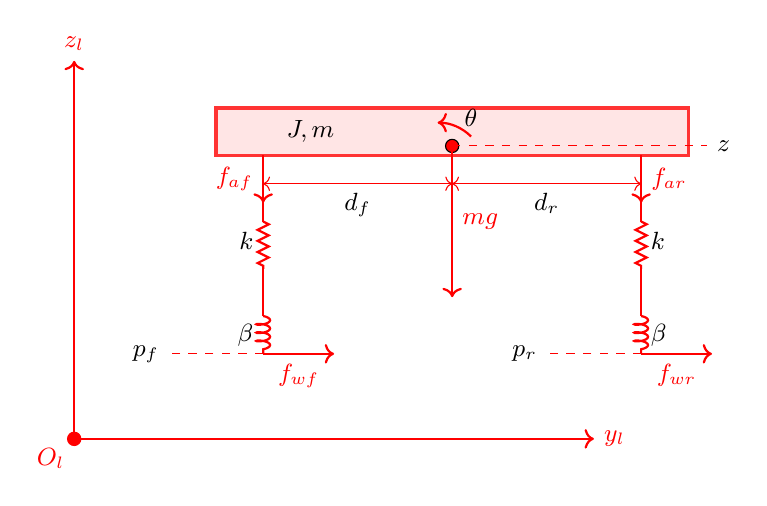
\begin{tikzpicture}[scale=1.2, every node/.style={font=\small}]
			
			% Coordinate axes
			\draw[->, thick, red] (-3.5,-1.5) -- (-3.5,2.5) node[above] {$z_l$};
			\draw[->, thick, red] (-3.5,-1.5) -- (2,-1.5) node[right] {$y_l$};
			\filldraw[red] (-3.5,-1.5) circle (2pt) node[below left] {$O_l$};
			
			% Sprung mass (body)
			\filldraw[color=red!80, fill=red!10, very thick] (-2,1.5) rectangle (3,2);
			\node at (-1,1.75) {$J, m$};
			
			% Center of mass
			\draw[fill=red] (0.5,1.6) circle (0.07);
			\draw[->, thick, red] (0.5,1.6) -- (0.5,0) node[midway,right] {$mg$};
			
			% pitch angle psi
			\draw[->, red, thick] (0,1.5) ++(0.7,0.2) arc[start angle=45,end angle=90,radius=0.5];
			\node at (0.7,1.9) {$\theta$};
			
			% Front suspension
			\draw[thick, red] (-1.5,1.5) -- (-1.5,0.8);
			\draw[thick, red, decorate, decoration={zigzag,segment length=4,amplitude=2}] (-1.5,0.8) -- (-1.5,0.3);
			\draw[thick, red] (-1.5,0.3) -- (-1.5,-0.2);
			\node[left] at (-1.5,0.6) {$k$};
			\draw[thick, red, decorate, decoration={coil,aspect=0.3, segment length=3}] (-1.5,-0.2) -- (-1.5,-0.6);
			\node[left] at (-1.5,-0.4) {$\beta$};
			\draw[->, thick, red] (-1.5,1.5) -- (-1.5,1.0) node[midway,left] {$f_{af}$};
			
			% Rear suspension
			\draw[thick, red] (2.5,1.5) -- (2.5,0.8);
			\draw[thick, red, decorate, decoration={zigzag,segment length=4,amplitude=2}] (2.5,0.8) -- (2.5,0.3);
			\draw[thick, red] (2.5,0.3) -- (2.5,-0.2);
			\node[right] at (2.5,0.6) {$k$};
			\draw[thick, red, decorate, decoration={coil,aspect=0.3, segment length=3}] (2.5,-0.2) -- (2.5,-0.6);
			\node[right] at (2.5,-0.4) {$\beta$};
			\draw[->, thick, red] (2.5,1.5) -- (2.5,1.0) node[midway,right] {$f_{ar}$};
			
			% Front and rear wheel forces
			\draw[->, thick, red] (-1.5,-0.6) -- (-0.75,-0.6) node[midway,below] {$f_{wf}$};
			\draw[->, thick, red] (2.5,-0.6) -- (3.25,-0.6) node[midway,below] {$f_{wr}$};
			
			% Ground heights
			\draw[dashed, red] (-1.5,-0.6) -- (-2.5,-0.6);
			\node[left] at (-2.5,-0.6) {$p_f$};
			\draw[dashed, red] (2.5,-0.6) -- (1.5,-0.6);
			\node[left] at (1.5,-0.6) {$p_r$};
			
			% Distances df and dr
			\draw[<->, red] (0.5,1.2) -- (-1.5,1.2);
			\node[below] at (-0.5,1.2) {$d_f$};
			\draw[<->, red] (0.5,1.2) -- (2.5,1.2);
			\node[below] at (1.5,1.2) {$d_r$};
			
			% Labels z
			\draw[dashed, red] (0.5,1.6) -- (3.2,1.6);
			\node[right] at (3.2,1.6) {$z$};
			
		\end{tikzpicture}
	\end{center}
	
	
%	
%	\begin{center}
%		
%		\begin{tikzpicture}[scale=1.2, every node/.style={font=\small}]
%			
%			% Coordinate axes
%			\draw[->, thick, red] (-3.5,-1.5) -- (-3.5,2.5) node[above] {$z_l$};
%			\draw[->, thick, red] (-3.5,-1.5) -- (2,-1.5) node[right] {$y_l$};
%			\filldraw[red] (-3.5,-1.5) circle (2pt) node[below left] {$O_l$};
%			
%			% Sprung mass (body)
%			\filldraw[color=red!80, fill=red!10, very thick] (-2,1.5) rectangle (3,2);
%			\node at (-1,1.75) {$J, m$};
%			
%			% Center of mass
%			\draw[fill=red] (0.5,1.6) circle (0.07);
%			\draw[->, thick, red] (0.5,1.6) -- (0.5,0) node[midway,right] {$mg$};
%			
%			% pitch angle theta
%			\draw[->, red, thick] (0,1.5) ++(0.7,0.2) arc[start angle=45,end angle=90,radius=0.5];
%			\node at (0.7,1.9) {$\theta$};
%			
%			% --- Front suspension ---
%			\draw[thick, red] (-1.5,1.5) -- (-1.5,0.8);
%			% Molla sospensione k
%			\draw[thick, red, decorate, decoration={zigzag,segment length=4,amplitude=2}] (-1.5,0.8) -- (-1.5,0.3);
%			\node[left] at (-1.5,0.6) {$k$};
%			\draw[thick, red] (-1.5,0.3) -- (-1.5,-0.1);
%			% Smorzatore beta
%			\draw[thick, red, decorate, decoration={coil,aspect=0.3, segment length=3}] (-1.5,-0.1) -- (-1.5,-0.5);
%			\node[left] at (-1.5,-0.3) {$\beta$};
%			\draw[thick, red] (-1.5,-0.5) -- (-1.5,-0.7);
%			% NUOVA: Molla pneumatico kt
%			\draw[thick, red, decorate, decoration={zigzag,segment length=4,amplitude=2}] (-1.5,-0.7) -- (-1.5,-1.2);
%			\node[left] at (-1.5,-0.95) {$k_t$};
%			\draw[thick, red] (-1.5,-1.2) -- (-1.5,-1.3);
%			
%			\draw[->, thick, red] (-1.5,1.5) -- (-1.5,1.0) node[midway,left] {$f_{af}$};
%			
%			% --- Rear suspension ---
%			\draw[thick, red] (2.5,1.5) -- (2.5,0.8);
%			% Molla sospensione k
%			\draw[thick, red, decorate, decoration={zigzag,segment length=4,amplitude=2}] (2.5,0.8) -- (2.5,0.3);
%			\node[right] at (2.5,0.6) {$k$};
%			\draw[thick, red] (2.5,0.3) -- (2.5,-0.1);
%			% Smorzatore beta
%			\draw[thick, red, decorate, decoration={coil,aspect=0.3, segment length=3}] (2.5,-0.1) -- (2.5,-0.5);
%			\node[right] at (2.5,-0.3) {$\beta$};
%			\draw[thick, red] (2.5,-0.5) -- (2.5,-0.7);
%			% NUOVA: Molla pneumatico kt
%			\draw[thick, red, decorate, decoration={zigzag,segment length=4,amplitude=2}] (2.5,-0.7) -- (2.5,-1.2);
%			\node[right] at (2.5,-0.95) {$k_t$};
%			\draw[thick, red] (2.5,-1.2) -- (2.5,-1.3);
%			
%			\draw[->, thick, red] (2.5,1.5) -- (2.5,1.0) node[midway,right] {$f_{ar}$};
%			
%			% Front and rear wheel forces (posizionate a fine kt)
%			\draw[->, thick, red] (-1.5,-1.3) -- (-0.75,-1.3) node[midway,below] {$f_{wf}$};
%			\draw[->, thick, red] (2.5,-1.3) -- (3.25,-1.3) node[midway,below] {$f_{wr}$};
%			
%			% Ground heights
%			\draw[dashed, red] (-1.5,-1.3) -- (-2.5,-1.3);
%			\node[left] at (-2.5,-1.3) {$p_f$};
%			\draw[dashed, red] (2.5,-1.3) -- (1.5,-1.3);
%			\node[left] at (1.5,-1.3) {$p_r$};
%			
%			% Distances df and dr
%			\draw[<->, red] (0.5,1.2) -- (-1.5,1.2);
%			\node[below] at (-0.5,1.2) {$d_f$};
%			\draw[<->, red] (0.5,1.2) -- (2.5,1.2);
%			\node[below] at (1.5,1.2) {$d_r$};
%			
%			% Labels z
%			\draw[dashed, red] (0.5,1.6) -- (3.2,1.6);
%			\node[right] at (3.2,1.6) {$z$};
%			
%		\end{tikzpicture}
		
		\begin{center}
	
		
		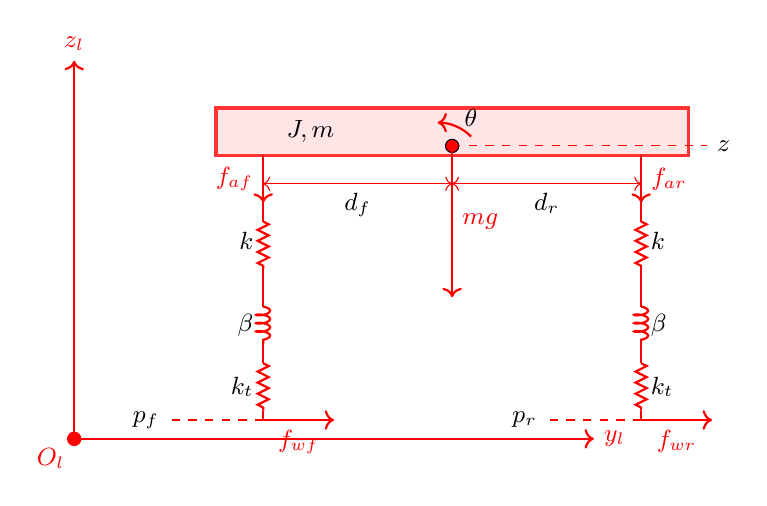
\begin{tikzpicture}[scale=1.2, every node/.style={font=\small}]
		
		% Coordinate axes
		\draw[->, thick, red] (-3.5,-1.5) -- (-3.5,2.5) node[above] {$z_l$};
		\draw[->, thick, red] (-3.5,-1.5) -- (2,-1.5) node[right] {$y_l$};
		\filldraw[red] (-3.5,-1.5) circle (2pt) node[below left] {$O_l$};
		
		% Sprung mass (body)
		\filldraw[color=red!80, fill=red!10, very thick] (-2,1.5) rectangle (3,2);
		\node at (-1,1.75) {$J, m$};
		
		% Center of mass
		\draw[fill=red] (0.5,1.6) circle (0.07);
		\draw[->, thick, red] (0.5,1.6) -- (0.5,0) node[midway,right] {$mg$};
		
		% pitch angle theta
		\draw[->, red, thick] (0,1.5) ++(0.7,0.2) arc[start angle=45,end angle=90,radius=0.5];
		\node at (0.7,1.9) {$\theta$};
		
		% --- Front suspension ---
		\draw[thick, red] (-1.5,1.5) -- (-1.5,0.8);
		% Molla sospensione k
		\draw[thick, red, decorate, decoration={zigzag,segment length=4,amplitude=2}] (-1.5,0.8) -- (-1.5,0.3);
		\node[left] at (-1.5,0.6) {$k$};
		\draw[thick, red] (-1.5,0.3) -- (-1.5,-0.1);
		% Smorzatore beta
		\draw[thick, red, decorate, decoration={coil,aspect=0.3, segment length=3}] (-1.5,-0.1) -- (-1.5,-0.5);
		\node[left] at (-1.5,-0.3) {$\beta$};
		\draw[thick, red] (-1.5,-0.5) -- (-1.5,-0.7);
		% NUOVA: Molla pneumatico kt
		\draw[thick, red, decorate, decoration={zigzag,segment length=4,amplitude=2}] (-1.5,-0.7) -- (-1.5,-1.2);
		\node[left] at (-1.5,-0.95) {$k_t$};
		\draw[thick, red] (-1.5,-1.2) -- (-1.5,-1.3);
		
		\draw[->, thick, red] (-1.5,1.5) -- (-1.5,1.0) node[midway,left] {$f_{af}$};
		
		% --- Rear suspension ---
		\draw[thick, red] (2.5,1.5) -- (2.5,0.8);
		% Molla sospensione k
		\draw[thick, red, decorate, decoration={zigzag,segment length=4,amplitude=2}] (2.5,0.8) -- (2.5,0.3);
		\node[right] at (2.5,0.6) {$k$};
		\draw[thick, red] (2.5,0.3) -- (2.5,-0.1);
		% Smorzatore beta
		\draw[thick, red, decorate, decoration={coil,aspect=0.3, segment length=3}] (2.5,-0.1) -- (2.5,-0.5);
		\node[right] at (2.5,-0.3) {$\beta$};
		\draw[thick, red] (2.5,-0.5) -- (2.5,-0.7);
		% NUOVA: Molla pneumatico kt
		\draw[thick, red, decorate, decoration={zigzag,segment length=4,amplitude=2}] (2.5,-0.7) -- (2.5,-1.2);
		\node[right] at (2.5,-0.95) {$k_t$};
		\draw[thick, red] (2.5,-1.2) -- (2.5,-1.3);
		
		\draw[->, thick, red] (2.5,1.5) -- (2.5,1.0) node[midway,right] {$f_{ar}$};
		
		% Front and rear wheel forces (posizionate a fine kt)
		\draw[->, thick, red] (-1.5,-1.3) -- (-0.75,-1.3) node[midway,below] {$f_{wf}$};
		\draw[->, thick, red] (2.5,-1.3) -- (3.25,-1.3) node[midway,below] {$f_{wr}$};
		
		% Ground heights
		\draw[dashed, red] (-1.5,-1.3) -- (-2.5,-1.3);
		\node[left] at (-2.5,-1.3) {$p_f$};
		\draw[dashed, red] (2.5,-1.3) -- (1.5,-1.3);
		\node[left] at (1.5,-1.3) {$p_r$};
		
		% Distances df and dr
		\draw[<->, red] (0.5,1.2) -- (-1.5,1.2);
		\node[below] at (-0.5,1.2) {$d_f$};
		\draw[<->, red] (0.5,1.2) -- (2.5,1.2);
		\node[below] at (1.5,1.2) {$d_r$};
		
		% Labels z
		\draw[dashed, red] (0.5,1.6) -- (3.2,1.6);
		\node[right] at (3.2,1.6) {$z$};
		
		\end{tikzpicture}
	\end{center}
	
	
	
	
	\textbf{todo: finire sto disegno}

	
	\begin{center} 
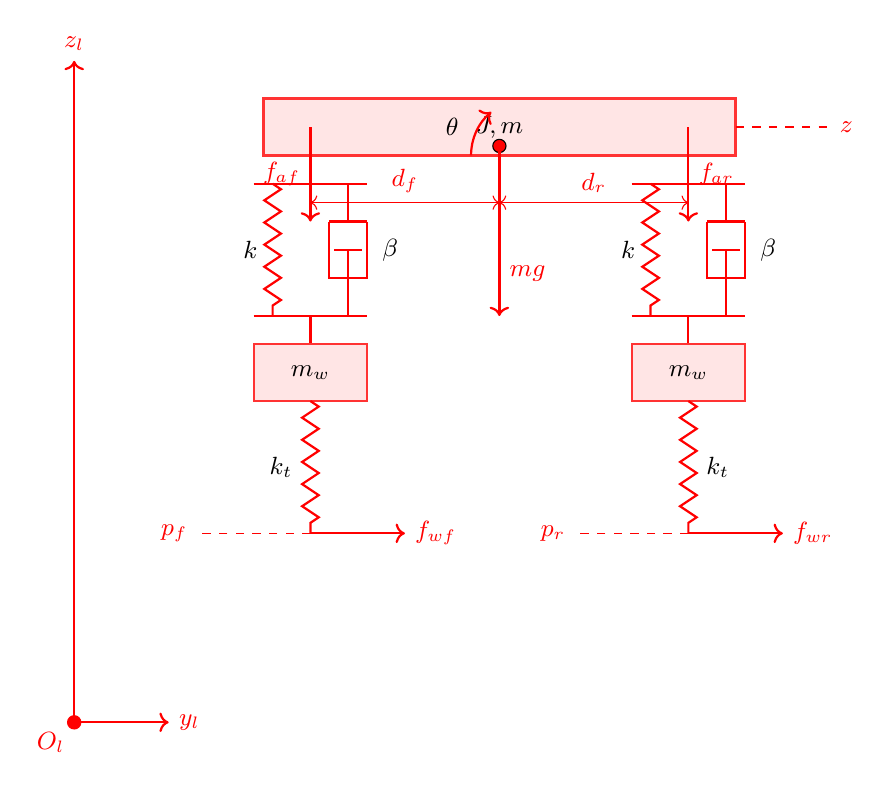
\begin{tikzpicture}[scale=1.2, every node/.style={font=\small}]
	% Coordinate axes - Spostati per non interferire
	\draw[->, thick, red] (-4,-3.5) -- (-4,3.5) node[above] {$z_l$};
	\draw[->, thick, red] (-4,-3.5) -- (-3,-3.5) node[right] {$y_l$};
	\filldraw[red] (-4,-3.5) circle (2pt) node[below left] {$O_l$};
	
	% --- SPRUNG MASS (Body) ---
	\filldraw[color=red!80, fill=red!10, very thick] (-2,2.5) rectangle (3,3.1);
	\node at (0.5,2.8) {$J, m$};
	
	% CM and Gravity
	\draw[fill=red] (0.5,2.6) circle (0.07);
	\draw[->, thick, red] (0.5,2.6) -- (0.5,0.8) node[right, near end] {$mg$};
	
	% Pitch angle theta
	\draw[->, red, thick] (0.2,2.5) arc[start angle=180, end angle=130, radius=0.6];
	\node at (0,2.8) {$\theta$};
	
	% --- FRONT SUSPENSION (Left) ---
	\def\xf{-1.5}
	% Connection to body
	\draw[thick, red] (\xf,2.5) -- (\xf,2.2);
	\draw[thick, red] (\xf-0.6,2.2) -- (\xf+0.6,2.2);
	
	% Sospensione superiore (k e beta parallelo) - DISTESA
	\draw[thick, red, decorate, decoration={zigzag,segment length=8,amplitude=3}] (\xf-0.4,2.2) -- (\xf-0.4,0.8);
	\node[left=2pt] at (\xf-0.4,1.5) {$k$};
	
	% Damper (beta)
	\draw[thick, red] (\xf+0.4,2.2) -- (\xf+0.4,1.8);
	\draw[thick, red] (\xf+0.2,1.8) -- (\xf+0.6,1.8); % Top cylinder
	\draw[thick, red] (\xf+0.2,1.8) -- (\xf+0.2,1.2) -- (\xf+0.6,1.2) -- (\xf+0.6,1.8); % Cylinder body
	\draw[thick, red] (\xf+0.25,1.5) -- (\xf+0.55,1.5); % Piston
	\draw[thick, red] (\xf+0.4,1.5) -- (\xf+0.4,0.8); % Rod
	\node[right=2pt] at (\xf+0.6,1.5) {$\beta$};
	
	\draw[thick, red] (\xf-0.6,0.8) -- (\xf+0.6,0.8);
	\draw[thick, red] (\xf,0.8) -- (\xf,0.5);
	
	% UNSPRUNG MASS (mw)
	\filldraw[color=red!80, fill=red!10, thick] (\xf-0.6,-0.1) rectangle (\xf+0.6,0.5);
	\node at (\xf, 0.2) {$m_w$};
	
	% TIRE STIFFNESS (kt) - DISTESA
	\draw[thick, red, decorate, decoration={zigzag,segment length=8,amplitude=3}] (\xf,-0.1) -- (\xf,-1.5);
	\node[left=3pt] at (\xf,-0.8) {$k_t$};
	
	% --- REAR SUSPENSION (Right) ---
	\def\xr{2.5}
	% Connection to body
	\draw[thick, red] (\xr,2.5) -- (\xr,2.2);
	\draw[thick, red] (\xr-0.6,2.2) -- (\xr+0.6,2.2);
	
	% Sospensione superiore (k e beta parallelo)
	\draw[thick, red, decorate, decoration={zigzag,segment length=8,amplitude=3}] (\xr-0.4,2.2) -- (\xr-0.4,0.8);
	\node[left=2pt] at (\xr-0.4,1.5) {$k$};
	
	% Damper (beta)
	\draw[thick, red] (\xr+0.4,2.2) -- (\xr+0.4,1.8);
	\draw[thick, red] (\xr+0.2,1.8) -- (\xr+0.6,1.8); 
	\draw[thick, red] (\xr+0.2,1.8) -- (\xr+0.2,1.2) -- (\xr+0.6,1.2) -- (\xr+0.6,1.8); 
	\draw[thick, red] (\xr+0.25,1.5) -- (\xr+0.55,1.5); 
	\draw[thick, red] (\xr+0.4,1.5) -- (\xr+0.4,0.8); 
	\node[right=2pt] at (\xr+0.6,1.5) {$\beta$};
	
	\draw[thick, red] (\xr-0.6,0.8) -- (\xr+0.6,0.8);
	\draw[thick, red] (\xr,0.8) -- (\xr,0.5);
	
	% UNSPRUNG MASS (mw)
	\filldraw[color=red!80, fill=red!10, thick] (\xr-0.6,-0.1) rectangle (\xr+0.6,0.5);
	\node at (\xr, 0.2) {$m_w$};
	
	% TIRE STIFFNESS (kt)
	\draw[thick, red, decorate, decoration={zigzag,segment length=8,amplitude=3}] (\xr,-0.1) -- (\xr,-1.5);
	\node[right=3pt] at (\xr,-0.8) {$k_t$};
	
	% --- FORCES AND GROUND ---
	% Ground forces
	\draw[->, thick, red] (\xf,-1.5) -- (\xf+1,-1.5) node[right] {$f_{wf}$};
	\draw[->, thick, red] (\xr,-1.5) -- (\xr+1,-1.5) node[right] {$f_{wr}$};
	
	% Ground inputs pf, pr
	\draw[dashed, red] (\xf,-1.5) -- (\xf-1.2,-1.5) node[left] {$p_f$};
	\draw[dashed, red] (\xr,-1.5) -- (\xr-1.2,-1.5) node[left] {$p_r$};
	
	% Distances df, dr
	\draw[<->, red] (0.5,2.0) -- (\xf,2.0) node[midway,above] {$d_f$};
	\draw[<->, red] (0.5,2.0) -- (\xr,2.0) node[midway,above] {$d_r$};
	
	% Active forces f_af, f_ar
	\draw[->, thick, red] (\xf,2.8) -- (\xf,1.8) node[midway,left] {$f_{af}$};
	\draw[->, thick, red] (\xr,2.8) -- (\xr,1.8) node[midway,right] {$f_{ar}$};
	
	% Reference height
	\draw[dashed, red] (3,2.8) -- (4,2.8) node[right] {$z$};
\end{tikzpicture}
	\end{center}
	Copy and past the Simulink block scheme and describe what each block does. Describe the set-up MATLAB file, where and how to change the parameters of the simulations. Remember to include also the sensor noises and realistic external disturbances.
	
	\section{Simulation results}
	Describe the simulation scenario: initial conditions, purpose of the simulation. Describe the results: are the results coherent with the expectation? If not why? Investigate the tuning: how the performance are affected by the selection of the parameters at disposal of the designer?
	
	\chapter{Conclusions and further investigation}
	Recap the main results obtained in the project and highlight eventual further investigation directions alogn which the performance could be improved. 
	
	\newpage
	\chapter*{Bibliography}
	List the papers/books cited.
	
	
	\newpage
	\appendix
	\chapter*{Appendix}
	Use appendices to add technical parts which are instrumental for the completeness of the manuscript but are too heavy to be included inside the main text. Basically, appendices are exploited to let the main text cleaner and smoother. As example, the complete MATLAB listings can be reported in appendix.\\
	
	
\end{document}          
